% =============================================================================
%  main.tex - preambulo, portada y \input de las secciones.
%
%  ESTE ARCHIVO ES DE TODO EL EQUIPO. Casi nunca debe cambiar: solo se toca
%  para agregar una seccion nueva al final (un \input mas).
%  Tu texto va en secciones/<tu-seccion>.tex.
%
%  Compilar desde esta carpeta:   latexmk        (el .latexmkrc ya hace el resto)
% =============================================================================

% nonatbib: elsarticle carga natbib por default y natbib es INCOMPATIBLE con
% biblatex. Esta opcion le dice a la clase que no lo cargue.
% 5p = formato Elsevier a dos columnas. Si lo quieren a una columna, cambien
% 5p por 3p y no hay que tocar nada mas.
\documentclass[5p,nonatbib]{elsarticle}

% --- Quitar el pie de pagina "Preprint submitted to Elsevier" -----------------
% No estamos mandando esto a una revista, es un reporte de clase.
\makeatletter
\def\ps@pprintTitle{%
  \let\@oddhead\@empty
  \let\@evenhead\@empty
  \let\@oddfoot\@empty
  \let\@evenfoot\@empty}
\makeatother

% --- Codificacion y tipografia -----------------------------------------------
\usepackage[T1]{fontenc}      % acentos y "ñ" como un solo glifo (permite copiar
                              % texto del PDF y que la division silabica sirva)
\usepackage[utf8]{inputenc}   % el .tex se escribe en UTF-8
                              % Sin paquete de tipografia: se usa la default de
                              % LaTeX (Computer Modern). Ojo: NO usar la opcion
                              % [times] de la clase, que la cambiaria.

\usepackage{microtype}        % micro-ajustes de espaciado; menos renglones feos

% A dos columnas las columnas son angostas y una palabra larga sin guiones
% (una ruta como references.bib, o un \verb) se sale del margen. Esto deja que
% LaTeX estire un poco los espacios antes de rendirse y desbordar.
\emergencystretch=2em

% --- Idioma ------------------------------------------------------------------
% Los ajustes de babel-spanish NO se pueden poner como opciones de \usepackage:
% babel leeria "es-tabla" como si fuera un idioma y truena. Van aqui, en
% \spanishoptions, ANTES de cargar babel.
%   es-tabla        -> "Tabla 1" en vez de "Cuadro 1"
%   es-nodecimaldot -> deja el punto decimal en matematicas (12.46 y no 12,46),
%                      porque asi salen los numeros de pandas/R
%   es-noquoting    -> evita que babel se pelee con otros paquetes por comillas
\def\spanishoptions{es-tabla,es-nodecimaldot,es-noquoting}
\usepackage[spanish]{babel}
\usepackage{csquotes}         % \enquote{...} -> «...» segun el idioma activo

% --- Matematicas -------------------------------------------------------------
\usepackage{amsmath}
\usepackage{amssymb}
\usepackage{amsthm}

% --- Tablas y figuras --------------------------------------------------------
\usepackage{booktabs}         % \toprule \midrule \bottomrule (tablas sin lineas
                              % verticales, que es el estilo correcto)
\usepackage{multirow}
\usepackage{graphicx}
\usepackage{multicol}
\graphicspath{{figuras/}}     % con esto basta \includegraphics{archivo.pdf}

% A dos columnas, un table* [t] cerca del final del documento puede empujar
% el resto del texto a una pagina nueva; si lo que queda despues no llena
% esa pagina, una columna se queda vacia. flushend balancea las dos columnas
% de la ULTIMA pagina para que ese sobrante no se vea como espacio en blanco.
\usepackage{flushend}


% El reporte tiene muchas tablas grandes (sobre todo en el diccionario de
% datos); el espaciado por defecto de LaTeX alrededor de flotantes y listas
% deja demasiado blanco. Se aprieta aqui para que el documento se vea mas
% denso sin tocar el tamano de fuente ni los margenes de la clase.
\setlength{\intextsep}{6pt plus 2pt minus 2pt}
\setlength{\textfloatsep}{8pt plus 2pt minus 2pt}
\setlength{\floatsep}{6pt plus 2pt minus 2pt}
\setlength{\abovecaptionskip}{4pt}
\setlength{\belowcaptionskip}{2pt}

% Parametros de colocacion de flotantes. Los defaults de LaTeX son
% conservadores y en este reporte se quedan cortos: la etapa 2 aporta 24
% flotantes contra unas 5 paginas de prosa, y como cada uno solo puede
% aparecer en o despues del punto donde se cita, la cola se desbordaba al
% final del documento (seis figuras quedaban DESPUES de la bibliografia).
%
% Lo que estorbaba, en concreto:
%   \textfraction 0.2 -> exigia que al menos 20%% de cada pagina fuera texto
%   \topnumber    2   -> maximo dos flotantes en la zona superior
%   \floatpagefraction 0.5 -> una pagina solo de flotantes tenia que ir medio
%                             llena, si no LaTeX prefiere seguir difiriendolos
%
% Esto NO recorta contenido ni cambia el tamano de letra: solo autoriza a
% LaTeX a empaquetar los flotantes mas densamente. Bajo el documento de 13 a
% 12 paginas y dejo la bibliografia al final, que es donde debe estar.
% Si en algun momento el reporte se ve demasiado saturado de figuras por
% pagina, estos son los diales que hay que aflojar (subir \textfraction,
% bajar \topnumber).
\renewcommand{\topfraction}{0.92}
\renewcommand{\bottomfraction}{0.6}
\renewcommand{\textfraction}{0.06}
\renewcommand{\floatpagefraction}{0.55}
\renewcommand{\dbltopfraction}{0.92}      %% idem para flotantes de ancho completo
\renewcommand{\dblfloatpagefraction}{0.55}
\setcounter{topnumber}{4}
\setcounter{bottomnumber}{3}
\setcounter{totalnumber}{6}
\setcounter{dbltopnumber}{3}

\usepackage{enumitem}
\setlist{noitemsep, topsep=3pt, partopsep=0pt}

% --- Bibliografia (biblatex + biber) -----------------------------------------
% style=authoryear -> (Jolliffe, 2002) en el texto.
% Para citas numericas [1], cambien authoryear por numeric-comp.
\usepackage[backend=biber,style=apa,sorting=nyt,maxbibnames=99]{biblatex}
\addbibresource{references.bib}
% La bibliografia se compone un punto mas chica que el cuerpo, convencion
% habitual en revistas: son datos de consulta, no prosa que se lea seguida.
% Con las URLs largas de las fuentes normativas esto ahorra ~10 renglones,
% que es lo que hacia que se derramara a una pagina extra.
\renewcommand*{\bibfont}{\small}
\setlength{\bibitemsep}{0pt}      %% sin aire extra entre entradas
\setlength{\bibhang}{1em}

% --- Referencias cruzadas (SIEMPRE hasta el final) ---------------------------
\usepackage[colorlinks=true, linkcolor=blue,citecolor=blue]{hyperref}
\usepackage[spanish]{cleveref} % \cref{fig:x} escribe solo "Figura 1"

\usepackage{mhchem} % formulas de quimica

% cleveref en español dice "apartado 2"; en un reporte queremos "Sección 2".
% \cref -> minuscula (a media oracion), \Cref -> mayuscula (al inicio).
\crefname{section}{sección}{secciones}
\Crefname{section}{Sección}{Secciones}
\crefname{table}{tabla}{tablas}
\Crefname{table}{Tabla}{Tablas}
\crefname{equation}{ecuación}{ecuaciones}
\Crefname{equation}{Ecuación}{Ecuaciones}

% --- Textos de la portada en español ----------------------------------------
% elsarticle trae "Abstract" y "Keywords" escritos a fuerza en ingles;
% la clase deja estos dos ganchos para cambiarlos.
\abstracttitle{Resumen}
\keywordtitle{Palabras clave}

\begin{document}

% --- Carátula ----------------------------------------------------------------
% La rúbrica pide número de equipo, nombre y matrícula de cada integrante y el
% nombre del proyecto vinculado con el objetivo. elsarticle no trae carátula,
% así que se compone a mano antes del frontmatter (que pone el resumen).
\begin{titlepage}
  \centering
  \vspace*{2cm}
  {\large Instituto Tecnológico y de Estudios Superiores de Monterrey\par}
  \vspace{0.4cm}
  {\large MA2003B --- Aplicación de Métodos Multivariados en Ciencia de Datos\par}
  {\large Grupo 102\par}
  \vspace{2.5cm}
  {\LARGE\bfseries Discriminación de excedencias diarias de ozono en el Área
    Metropolitana de Monterrey\par}
  \vspace{0.6cm}
  {\large Clasificación día-estación bajo el umbral de 51 ppb de la
    NOM-020-SSA1-2021 con análisis factorial, regresión logística,
    discriminante lineal y modelo autorregresivo, sobre 15 estaciones del
    SIMA, 2021--2025\par}
  \vspace{2.5cm}
  {\large\bfseries Equipo 7\par}
  \vspace{0.5cm}
  \begin{tabular}{ll}
    \toprule
    Integrante & Matrícula \\
    \midrule
    Eduardo Luna    & \texttt{A00842657} \\
    Jenaro Alcaraz  & \texttt{A01646850} \\
    Emilia Rico     & \texttt{A01384587} \\
    Mar Fernández   & \texttt{A00227571} \\
    Sofía Fernández & \texttt{A01722980} \\
    \bottomrule
  \end{tabular}
  \vfill
  {\large Monterrey, Nuevo León\par}
  {\large Septiembre de 2026\par}
\end{titlepage}

\begin{frontmatter}

\title{Discriminación de excedencias diarias de ozono en el Área Metropolitana
de Monterrey\\
\large Clasificación día-estación bajo el umbral de 51 ppb de la
NOM-020-SSA1-2021 en 15 estaciones del SIMA, 2021--2025}

\author[tec]{Eduardo Luna}
\author[tec]{Jenaro Alcaraz}
\author[tec]{Emilia Rico}
\author[tec]{Mar Fernández}
\author[tec]{Sofía Fernández}
\address[tec]{Instituto Tecnológico y de Estudios Superiores de Monterrey, MA2003B --- Grupo 102, equipo 7}

% Resumen de una página a espacio sencillo, como pide la rúbrica: problema,
% datos, método, resultado. Sin citas, fórmulas ni referencias a secciones.
\begin{abstract}
El ozono troposférico del Área Metropolitana de Monterrey excede con
regularidad el límite que la NOM-020-SSA1-2021 fija para el máximo diario de
la media móvil de 8 horas (MDA8), y la tendencia de las últimas tres décadas
es al alza, en contraste con la de la Ciudad de México. Este trabajo se
pregunta qué condiciones meteorológicas y de contaminantes primarios
acompañan a un día de excedencia, y qué tan bien se puede discriminar ese día
a partir de ellas. Se adopta como respuesta la indicadora de excedencia del
MDA8 sobre 51 ppb, la meta a 5 años de la norma, porque con el umbral vigente
de 65 ppb las excedencias son 11.25\,\% de los días-estación y un
clasificador constante alcanzaría 88.75\,\% de exactitud sin identificar el
fenómeno.

Los datos son los registros horarios de las 15 estaciones del Sistema
Integral de Monitoreo Ambiental de Nuevo León entre el 1 de enero de 2021 y
el 31 de diciembre de 2025: ocho contaminantes criterio y siete parámetros
meteorológicos. El año 2020 se descarta por faltantes superiores a 89\,\% en
siete estaciones. Las series se limpian de valores centinela y físicamente
imposibles, se transforman con Box-Cox para llevar el sesgo por debajo de
0.5 en valor absoluto, se estandarizan y se agregan a una fila por
día-estación con 16 resúmenes diarios; 25,100 filas cuentan con MDA8 válido.
Los años 2021--2024 se destinan al ajuste y 2025 completo a la validación,
sin que ningún procedimiento vea el segundo.

La modelación combina técnicas de interdependencia y de dependencia. El
análisis de componentes principales retiene tres ejes con 55.9\,\% de la
varianza y los identifica como carga primaria de combustión, forzamiento
fotoquímico y estancamiento atmosférico. El análisis factorial exploratorio,
sobre 13 predictores tras retirar dos redundancias que produjeron
comunalidades imposibles, recupera tres factores ortogonales ---combustión
primaria, ventilación y forzamiento fotoquímico--- que explican 40.3\,\% de
la varianza común y reaparecen en 2025 con congruencia de Tucker superior a
0.92. Sobre esos tres puntajes y 12 indicadoras de zona, tipo de día y
temporada se ajustan una regresión logística y un análisis discriminante
lineal. Ambos superan el criterio de logro de 0.75 en el área bajo la curva
ROC, con 0.850 y 0.846 en 2025; la diferencia es estadísticamente detectable
pero sin consecuencia práctica, de modo que la interpretación de las razones
de momios no depende del supuesto de normalidad que el discriminante exige.
Una desviación estándar adicional de forzamiento fotoquímico multiplica los
momios de excedencia por 2.78 y una de combustión primaria por 1.92; la
ventilación es el único factor protector (0.90). La primavera triplica los
momios respecto al invierno y las zonas Noroeste y Suroeste los triplican
respecto al Noreste. Los errores estándar corregidos por conglomerado de día
se inflan hasta 2.5 veces y las conclusiones se sostienen, salvo el efecto
del sábado.

La caracterización de los puntajes como series de tiempo muestra que la
autocorrelación de un día para otro sobrevive a la descomposición estacional,
lo que motiva un modelo autorregresivo logístico sobre la serie diaria de
área metropolitana. Con un solo rezago de la respuesta, los tres factores y
los armónicos del calendario, alcanza un AUC de 0.898 en 2025 y supera a la
climatología (0.668) y a la persistencia (0.717); haber excedido el día
anterior multiplica los momios por 3.83. La validación cruzada por año sitúa
la generalización esperada en 0.878 y revela un efecto de año ---2024 y 2025
son los de ozono más alto de la serie--- que ningún predictor explica y que
queda como la limitación principal, junto con la ausencia de mediciones de
compuestos orgánicos volátiles, que impide atribuir un régimen fotoquímico.
Los resultados indican que la excedencia es un fenómeno estacional y
regional modulado por el viento, con una señal espacial en el poniente de la
ciudad que no explica la meteorología medida.
\end{abstract}

\begin{keyword}
ozono troposférico \sep análisis factorial \sep análisis de componentes
principales \sep regresión logística \sep análisis discriminante lineal \sep
modelo autorregresivo \sep Área Metropolitana de Monterrey
\end{keyword}

\end{frontmatter}

% --- Secciones ---------------------------------------------------------------
% Una seccion = un archivo = una issue = una branch.
% El orden sigue la rubrica del curso: introduccion y justificacion,
% problematica y objetivo, preparacion de la base de datos, modelacion y
% validacion, resultados, discusion y conclusiones. Cada archivo de
% secciones/ abre con el nivel de encabezado que le toca aqui; al mover un
% archivo de lugar hay que revisar ese nivel.

% 1. Introducción y justificación
% Seccion 1 de la rubrica: introduccion y justificacion. Abre con \section y
% aloja como \subsection a revi_medio_ambiente.tex, res_sima.tex y
% contexto_estaciones.tex, que se \input inmediatamente despues en main.tex.
% El objeto de investigacion (el ozono) vivia en objetivo.tex; se fusiono aqui
% porque es justificacion, no objetivo.

\section{Introducción y justificación}
\label{sec:introduccion}

La calidad del aire en Nuevo León es un factor determinante de la salud
pública: la exposición diaria a concentraciones elevadas de contaminantes
representa un riesgo acumulativo para la población. Las mediciones continuas
del Sistema Integral de Monitoreo Ambiental (SIMA), descrito en la
\cref{sec:sima}, permiten caracterizar la atmósfera del Área Metropolitana
de Monterrey (AMM) y son la fuente de este trabajo. Para reportar la calidad
del aire, SIMA convierte las mediciones horarias en un índice categórico con
un color asociado a su valor máximo \parencite{aireNL2026}.

De los contaminantes que mide la red, el ozono troposférico es el que
justifica este estudio: es secundario, no se emite sino que se forma, y su
formación depende a la vez de los precursores químicos y de las condiciones
meteorológicas. Esa doble dependencia es lo que vuelve pertinente un análisis
multivariado: ninguna variable por sí sola explica un día de excedencia.

\subsection{El ozono troposférico}
\label{sec:objetivo}

El ozono \ce{O3} es una sustancia compuesta por tres átomos de oxígeno que se
encuentra tanto en la atmósfera superior (ozono estratosférico) como a nivel
del suelo (ozono troposférico). El estratosférico se produce de manera
natural por la interacción entre el oxígeno molecular \ce{O2} y los rayos
ultravioleta, y atenúa la exposición de la superficie a esa radiación
\parencite{Bernhard2023-lk}. El troposférico, en cambio, es el principal
ingrediente del \textit{smog} y se forma por transformaciones químicas entre
los óxidos de nitrógeno \ce{NOx} y los compuestos orgánicos volátiles (COV)
con el calor y la luz solar.

Áreas metropolitanas de Nuevo León con elevada actividad industrial han
presentado niveles de \ce{O3} y \ce{PM10} que superan los límites de la
NOM-020-SSA1-2021 \parencite{nom020ssa1} y la NOM-025-SSA1-2014
\parencite{nom025ssa1}. Estas tendencias se documentan desde hace más de
30 años, con herramientas que miden tanto el ozono (fotometría ultravioleta)
como sus precursores \ce{NO} y \ce{NO2} (agrupados como \ce{NO_x}, por
quimioluminiscencia), cuya relación fotoquímica es clave para entender la
formación del contaminante secundario \parencite{SanfordSillman}.

El AMM no es la excepción: entre 1993 y 2014 se registró un aumento
sostenido de las concentraciones de ozono troposférico, en contraste con la
tendencia descendente de la Ciudad de México en el mismo periodo, atribuido
al crecimiento industrial y vehicular sin un control equivalente sobre los
precursores y a un papel meteorológico modulado por el cambio climático
\parencite{atmos15070779}. El comportamiento se agrava por la topografía del
valle donde se asienta el AMM, rodeado de sierras que favorecen el
estancamiento de masas de aire durante episodios de alta presión, inversión
térmica y viento débil, factores que reducen la dispersión y prolongan la
exposición de la población.
          % \section + el ozono
\section{Revisión de medio ambiente y salud}

\subsection{Estudio de impactos en la salud por contaminantes}

El análisis de la calidad del aire es importante para la ciudadanía, porque la
contaminación atmosférica representa un riesgo para la salud y se relaciona
con enfermedades como cardiopatías, accidentes cerebrovasculares, neumonía,
cáncer de pulmón e infecciones respiratorias. Este estudio analiza diversos
contaminantes \parencite{oms2021}:

\begin{itemize}
	\item partículas suspendidas \ce{PM2.5} y \ce{PM10};
	\item dióxido de nitrógeno (\ce{NO2});
	\item ozono (\ce{O3}); y
	\item dióxido de azufre (\ce{SO2}).
\end{itemize}

También considera sus concentraciones, la exposición de la población y los
datos de salud. La calidad del aire se mide mediante estaciones de monitoreo
que registran concentraciones horarias, a partir de las cuales se calculan
métricas como promedios de 24 horas o anuales, dependiendo del contaminante.
El estudio utiliza normas oficiales mexicanas, como la NOM-025-SSA1-2021 para
\ce{PM2.5}, y las compara con las recomendaciones de la Organización Mundial
de la Salud (OMS).

Una problemática identificada es que algunos límites mexicanos son menos
estrictos que los recomendados por la OMS. Por ejemplo, para \ce{PM2.5}, el
límite mexicano es de $10\,\mu\mathrm{g}/\mathrm{m}^{3}$, mientras que la OMS
recomienda $5\,\mu\mathrm{g}/\mathrm{m}^{3}$. Además, la medición enfrenta
dificultades porque no todas las estaciones miden todos los contaminantes ni
cuentan con suficientes datos válidos. Por ello, se requieren criterios de
suficiencia, como contar con al menos el 75\% de datos válidos
\parencite{nom025ssa1,oms2021}.

\subsection{Contaminación del aire doméstico: riesgos relativos}

Este documento informa sobre los efectos de la contaminación del aire en la
salud. Presenta riesgos importantes y su relación con diferentes enfermedades,
entre ellas infecciones respiratorias de vías aéreas inferiores, enfermedad
pulmonar obstructiva crónica, cáncer de pulmón, cardiopatía isquémica y
accidente cerebrovascular. También considera diferencias según la edad y el
sexo, y utiliza intervalos de confianza del 95\% para expresar la incertidumbre
de los resultados.

Por ejemplo, el riesgo relativo es particularmente elevado para el cáncer de
pulmón en mujeres. En conclusión, el documento muestra que analizar la
contaminación del aire es importante para conocer y cuantificar sus posibles
efectos sobre la salud de la población.

\subsection{Normativa de aire de Nuevo León}

Esta fuente permite conocer las normas oficiales y la interpretación de las
mediciones de calidad del aire. Las normas establecen límites de concentración
para diferentes contaminantes y consideran tanto la cantidad del contaminante
como el tiempo de exposición, ya que los límites pueden establecerse para
periodos de una hora, ocho horas, 24 horas o promedios anuales.

Por ejemplo, la Norma Oficial Mexicana NOM-021-SSA1-2021 evalúa la calidad del
aire ambiente con respecto al monóxido de carbono (\ce{CO}). La página reúne
12 normas oficiales mexicanas
\parencite{nlAirenlgobmxNormatividad,NOMCalidadAireAmbiente}.

Las mediciones permiten comparar la concentración registrada con los valores
establecidos en las normas para determinar si se cumplen los límites
correspondientes. La fuente confirma que los límites se establecen considerando
los posibles efectos sobre la salud, pero no desarrolla una clasificación
internacional de contaminantes.
   % \subsection
\section{Sistema Integral de Monitoreo Ambiental (SIMA)}
\label{sec:sima}

El Sistema Integral de Monitoreo Ambiental (SIMA) es la red del Gobierno de
Nuevo León encargada de medir y vigilar la calidad del aire. Su objetivo es
conocer las concentraciones de contaminantes a las que está expuesta la
población, generar alertas cuando existen condiciones de contaminación elevada
y mantener informados a los ciudadanos sobre la salud ambiental y la calidad del
aire \parencite{gobiernoNL2026PIGECA}.

SIMA inició operaciones el 20 de noviembre de 1992 como un departamento de la
Subsecretaría de Protección al Medio Ambiente y Recursos Naturales, con tan
solo cinco estaciones de monitoreo. Durante 32 años ha crecido y modernizado
su infraestructura \parencite{villasaez2024}. Actualmente cuenta con 15
estaciones fijas distribuidas estratégicamente en 11 municipios de la zona
metropolitana de Monterrey, además de 2 estaciones móviles
\parencite{gobiernoNL2026ModernizacionSIMA}.

SIMA mide ocho contaminantes criterio y siete parámetros meteorológicos,
detallados junto con sus unidades y cobertura en el diccionario de datos
(\cref{tab:dic-contaminantes,tab:dic-meteo}).

SIMA es la infraestructura gubernamental encargada de convertir la información
sobre la contaminación atmosférica en acciones de gestión ambiental, y es el
medio por el cual se obtiene una parte fundamental de la información necesaria
para hacerlo.

Los datos utilizados en este trabajo se relacionan directamente con SIMA, ya
que provienen de las mediciones realizadas por sus estaciones de monitoreo
ambiental. Las estaciones registran regularmente contaminantes y variables
meteorológicas. Una vez extraídos, los datos se procesan y validan para
integrarlos en las bases de datos de la institución.              % \subsection
% Continuacion de la introduccion (\subsection). Contexto geografico de las
% estaciones: la rubrica pide describir ubicacion y factores geograficos que
% podrian influir en las mediciones. Coordenadas y elevacion vienen del
% catalogo docs/Ubicacion de las estaciones de monitoreo.docx; la lectura
% espacial, de docs/05_estacionalidad_ozono.pdf.

\subsection{Las estaciones y su contexto geográfico}
\label{sec:contexto-estaciones}

El AMM ocupa un valle a unos 500 msnm limitado al sur y al poniente por la
Sierra Madre Oriental, al oriente por el Cerro de la Silla y al norte por el
Cerro del Topo Chico y la Sierra de las Mitras. Las 15 estaciones del SIMA se
reparten en ese valle a lo largo de un gradiente de elevación de 334 msnm,
en la planicie del sureste, a 702 msnm, al pie de la sierra en el noroeste
(\cref{tab:estaciones}). El código de cada estación indica su cuadrante, y a
partir de él se homologan en siete zonas que los modelos de
\cref{sec:clasificacion_tecs} usan como predictor categórico.

\begin{table}[t]
  \centering
  \caption{Estaciones del SIMA, zona a la que se homologan y elevación.
    Coordenadas en grados y minutos; todas en latitud norte y longitud
    oeste.}
  \label{tab:estaciones}
  \small
  \begin{tabular}{llrll}
    \toprule
    Código & Zona & msnm & Lat. & Long. \\
    \midrule
    \texttt{SE3}  & Sureste  & 334 & 25°36' & 100°00'  \\
    \texttt{NE3}  & Noreste  & 346 & 25°47' & 100°05' \\
    \texttt{SE2}  & Sureste  & 387 & 25°39' & 100°06' \\
    \texttt{NE2}  & Noreste  & 432 & 25°47' & 100°11' \\
    \texttt{NE}   & Noreste  & 474 & 25°45' & 100°15' \\
    \texttt{SE}   & Sureste  & 500 & 25°40' & 100°15' \\
    \texttt{NTE}  & Norte    & 503 & 25°48' & 100°20' \\
    \texttt{NTE2} & Norte    & 520 & 25°44' & 100°19' \\
    \texttt{SUR}  & Sur      & 555 & 25°37' & 100°16' \\
    \texttt{CE}   & Centro   & 562 & 25°41' & 100°20' \\
    \texttt{NO}   & Noroeste & 568 & 25°46' & 100°22' \\
    \texttt{NO3}  & Noroeste & 607 & 25°46' & 100°28' \\
    \texttt{SO2}  & Suroeste & 636 & 25°40' & 100°25' \\
    \texttt{SO}   & Suroeste & 674 & 25°41' & 100°27' \\
    \texttt{NO2}  & Noroeste & 702 & 25°48' & 100°35' \\
    \bottomrule
  \end{tabular}
\end{table}

Tres factores geográficos condicionan las mediciones. El primero es el
viento: la mediana de la componente zonal del viento es negativa (\cref{tab:cuartiles-iqr}), es decir, el
viento predominante entra del oriente y arrastra los precursores emitidos en
el centro y el oriente de la ciudad hacia el poniente, donde la sierra frena
su salida. El segundo es la elevación, que covaría con la distancia a las
fuentes de \ce{NOx} y con el uso de suelo: la correlación entre la elevación
de una estación y su tasa de excedencia es 0.827 sobre las 15 estaciones
(\cref{fig:elevacion-excedencia}). El tercero es el encierro orográfico ya
descrito en \cref{sec:objetivo}, que en episodios de alta presión y viento
débil impide la dispersión vertical y horizontal. El resultado es un
ordenamiento poniente--oriente estable en las cuatro temporadas: el Noroeste
y el Suroeste concentran las tasas de excedencia más altas (43.3\,\% y
42.1\,\%) y el Noreste la más baja (19.5\,\%).

\begin{figure}[t]
  \centering
  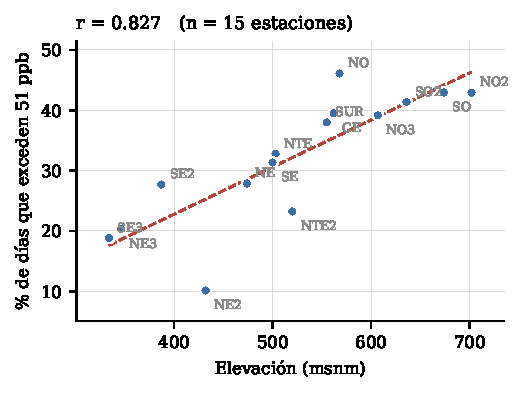
\includegraphics[width=\linewidth]{elevacion_vs_excedencia.pdf}
  \caption{Tasa de excedencia del MDA8 a 51 ppb contra elevación de cada
    estación, 2021--2025. Con $n=15$ y estaciones vecinas correlacionadas, la
    recta describe una asociación, no un efecto de la altitud.}
  \label{fig:elevacion-excedencia}
\end{figure}

Dos consideraciones acotan la comparabilidad entre estaciones.
\texttt{NO3} opera desde diciembre de 2022 y \texttt{NE3} entró en operación
después que el resto, de modo que su ventana es más corta; y ninguna estación
mide compuestos orgánicos volátiles, el segundo precursor del ozono, lo que
limita toda interpretación química a los óxidos de nitrógeno y al \ce{CO}
como sustituto.
   % \subsection

% 2. Problemática y objetivo
% Seccion 2 de la rubrica: problematica y objetivo. Fija el objetivo
% estadistico, las tecnicas y las variables. Las cifras que se citan aqui
% vienen del analisis exploratorio; se referencian con \cref, no se repiten.

\section{Problemática y objetivo}
\label{sec:objetivo-tecnicas}

\subsection{Problemática}

El AMM acumula tres décadas de ozono al alza (\cref{sec:objetivo}) y su red
de monitoreo produce, cada hora y en 15 puntos, las concentraciones de los
precursores y las condiciones meteorológicas que gobiernan su formación. La
pregunta que este trabajo responde es qué combinación de esas condiciones
acompaña a un día en que el ozono supera la norma, y con qué certeza puede
identificarse ese día a partir de ellas. Dos obstáculos la vuelven un
problema multivariado y no una comparación de umbrales: los precursores
están fuertemente correlacionados entre sí (\ce{NO}, \ce{NO2} y \ce{NOx} son
la misma emisión medida tres veces) y la respuesta es rara con el umbral
vigente, de modo que una regla trivial acierta casi siempre sin decir nada.

\subsection{Objetivo del análisis multivariado}
\label{sec:obj:objetivo}

\textbf{Objetivo principal.} Clasificar cada registro día-estación como
excedencia o no excedencia del MDA8 en el umbral de 51 ppb, a partir de los
precursores y variables meteorológicas del mismo día, e identificar qué
condiciones latentes explican esa clasificación.

\textit{Criterio de logro:} área bajo la curva ROC $\geq 0.75$ en una
partición de validación no vista durante el ajuste, con sensibilidad y
especificidad reportadas por separado. No se utiliza la exactitud: con el
umbral vigente de 65 ppb las excedencias son 11.25\,\% de los días-estación
válidos y un clasificador constante alcanzaría 88.75\,\% de exactitud sin
identificar el fenómeno (\cref{sec:eda-cualitativas}). Por esa razón el
escenario principal usa 51 ppb, la meta a 5 años de la NOM-020-SSA1-2021
(\cref{tab:nom-limites}), con 31.96\,\% de excedencias \parencite{saito2015}.

Las estaciones no se agrupan por sus niveles medios de ozono, que la
estación explica en apenas 5.3\,\% de la varianza del MDA8, sino que se
homologan en las siete zonas de \cref{sec:contexto-estaciones}, cuyo
contenido espacial sí se sostiene en los datos.

\subsection{Técnicas estadísticas}
\label{sec:obj:tecnicas}

Se combinan técnicas de interdependencia, que reducen los predictores a ejes
interpretables, con técnicas de dependencia, que relacionan esos ejes con la
excedencia:

\begin{itemize}
  \item \textbf{Análisis de componentes principales (ACP)}: resuelve la
    multicolinealidad de los predictores y produce ejes ortogonales con
    lectura física.
  \item \textbf{Análisis factorial exploratorio (AF)}: separa la varianza
    común de la específica y expone redundancias que el ACP absorbe sin
    señalar. Sus puntajes son los predictores de los modelos de
    clasificación.
  \item \textbf{Regresión logística}: modela la probabilidad de excedencia y
    el aporte de cada predictor como razón de momios, sin supuestos de
    normalidad; ya se ha aplicado a la excedencia del MDA8 a partir de
    variables meteorológicas \parencite{otero2016}.
  \item \textbf{Análisis discriminante lineal}: contrasta a la logística bajo
    los supuestos de normalidad multivariada y covarianzas iguales
    \parencite{hosmer2013}. Box-Cox dejó los sesgos en $|\text{sesgo}|<0.5$
    (\cref{tab:sesgos-transformacion}), lo que aproxima el primero.
  \item \textbf{Modelo autorregresivo logístico}: incorpora la dependencia
    temporal de la respuesta, que la caracterización como serie de tiempo
    muestra que persiste tras remover la estacionalidad.
\end{itemize}

Todos los clasificadores se evalúan con el área bajo la curva ROC, no con
exactitud, por el desbalance señalado \parencite{saito2015}. Se requiere la
estandarización de \cref{sec:transformaciones}: en unidades originales la
presión, con valores cercanos a 710, dominaría las distancias frente al
\ce{CO}, cuyos valores son menores que 10.

\subsection{Variables y sus características}
\label{sec:obj:variables}

Las definiciones, unidades y faltantes se encuentran en el diccionario de
datos (\cref{sec:diccionario}); la \cref{tab:variables-tecnica} presenta el
papel de cada grupo en el objetivo.

\begin{table}[t]
  \centering
  \caption{Papel de cada grupo de variables en el objetivo.}
  \label{tab:variables-tecnica}
  \footnotesize
  \begin{tabular}{p{3.4cm} p{4.4cm}}
    \toprule
    Grupo & Papel \\
    \midrule
    \ce{O3}, MDA8 & Definen la clase; no son predictores \\
    \addlinespace[2pt]
    \ce{NO}, \ce{NO2}, \ce{NO_x}, \ce{CO} & Predictores, ventana matutina
      06--09 h \parencite{abdulwahab2005} \\
    \addlinespace[2pt]
    \ce{PM10}, \ce{PM2.5}, \ce{SO2} & Predictores, media diaria \\
    \addlinespace[2pt]
    \texttt{TOUT}, \texttt{RH}, \texttt{SR}, \texttt{PRS}, \texttt{WSR},
      \texttt{viento\_u}, \texttt{viento\_v} & Predictores, resúmenes
      diarios (máximo, acumulado, media, mínimo) \\
    \addlinespace[2pt]
    \texttt{temporada}, \texttt{tipo\_dia}, \texttt{zona} & Predictores
      categóricos, codificados en $k-1$ indicadoras \\
    \bottomrule
  \end{tabular}
\end{table}

Los precursores se resumen en la ventana 06--09 h porque es la emisión
matutina la que alimenta la fotoquímica del mediodía; la radiación solar se
conserva para distinguir la atenuación por aerosol de una diferencia en la
disponibilidad de luz. Las categóricas entran con $k-1$ indicadoras y una
categoría de referencia explícita (Noreste, día laborable e invierno);
incluir los $k$ niveles generaría colinealidad perfecta con el término
independiente. El ACP y el AF excluyen estas indicadoras porque las columnas
binarias inflarían artificialmente la varianza explicada.


% 3. Preparación de la base de datos
\section{Preparación de la base de datos}
\label{sec:preparacion-datos}

\subsection{Consolidación y limpieza}

Los seis archivos anuales del SIMA no comparten estructura: cambian los
encabezados, la posición de la fila de unidades y el número de estaciones
(13 en 2020, 15 desde 2024). Se consolidan en una sola tabla horaria de 15
parámetros por estación y fecha, 754,603 registros entre 2020 y 2025. La
auditoría de calidad detecta valores centinela ($-9999$, el código de
faltante del registrador) y físicamente imposibles (humedad relativa de
hasta 725\,\%, temperaturas de 785\,°C), que se convierten a faltante en vez
de imputarse; el detalle está en el diccionario de datos
(\cref{sec:dic:centinela}). El porcentaje de faltantes por parámetro va de
3.66\,\% en la radiación solar a 25.23\,\% en \ce{PM2.5}, pero no se reparte
de forma pareja entre años ni estaciones, lo que determina la ventana de
estudio.

\subsection{Selección de datos}

A partir del diccionario de datos y del diagnóstico de calidad se construye
el conjunto de datos de los procesos subsiguientes.

Dado que el objetivo es analizar el comportamiento del ozono troposférico, se evalúa cada variable y se determina, con base en la literatura, si existe un mecanismo documentado por el cual influya en la formación de \ce{O3}, ya sea químico, físico o meteorológico.

Se fija como variable objetivo el \ce{O3} proveniente de la base de datos:

\begin{table*}[t]
  \centering
  \caption{Variable objetivo: ozono troposférico (\ce{O3}).}
  \label{tab:variable-objetivo}
  \begin{tabular}{lcccc}
    \toprule
    Unidad & Rango de operación & Rango observado & Mediana & Nulos (\%) \\
    \midrule
    ppb & 0--153 a 0--185 & 0.5--265.0 & 23.00 & 14.73 \\
    \bottomrule
  \end{tabular}
\end{table*}

\begin{quote}
    Las estaciones reportan resultados cada hora, lo que implica 24 mediciones diarias. La métrica normativa MDA8 colapsa esas 24 mediciones en un único valor por estación y día, ya que la NOM-020-SSA1 fija el límite de ozono sobre el promedio de 8 horas, no sobre el valor horario.
\end{quote}

El \cref{tab:nom-limites} reúne los valores límite vigentes en México para el
ozono y el material particulado. Nótese que el indicador normativo del \ce{O3} no
es la concentración horaria sino el promedio móvil de ocho horas, y que el
criterio de evaluación es el máximo de los máximos diarios de dichos promedios;
esto justifica adoptar el máximo diario del promedio móvil de ocho horas (MDA8)
como variable objetivo del análisis.

\begin{table*}[t]
  \centering
  \caption{Valores límite de calidad del aire vigentes en México para los
    contaminantes de interés. Los años indican el calendario de cumplimiento
    gradual establecido por cada norma
    \parencite{nom020ssa1, nom025ssa1}.}
  \label{tab:nom-limites}
  \footnotesize
  \begin{tabular}{p{2.6cm} p{7.2cm} ccc}
    \toprule
    & & \multicolumn{3}{c}{Valor límite} \\
    \cmidrule(lr){3-5}
    Indicador & Criterio de evaluación & Año 1 & Año 3 & Año 5 \\
    \midrule
    \multicolumn{5}{l}{\textbf{\ce{PM10}} ($\mu$g/m$^{3}$) --- NOM-025-SSA1-2021, DOF 27-oct-2021} \\
    \addlinespace[2pt]
    24 horas & Percentil 99 (frecuencia tolerada: 1\,\% de veces al año) & 70 & 60 & 50 \\
    Anual    & Promedio anual de los promedios de 24 horas              & 36 & 28 & 20 \\
    \midrule
    \multicolumn{5}{l}{\textbf{\ce{PM2.5}} ($\mu$g/m$^{3}$) --- NOM-025-SSA1-2021, DOF 27-oct-2021} \\
    \addlinespace[2pt]
    24 horas & Percentil 99 (frecuencia tolerada: 1\,\% de veces al año) & 41 & 33 & 25 \\
    Anual    & Promedio anual de los promedios de 24 horas              & 10 & 10 & 10 \\
    \midrule
    \multicolumn{5}{l}{\textbf{Ozono} (\ce{O3}, ppm) --- NOM-020-SSA1-2021, DOF 28-oct-2021} \\
    \addlinespace[2pt]
    1 hora                     & Máximo de los máximos diarios de las concentraciones horarias                        & 0,090 & 0,090 & 0,090 \\
    Promedio móvil de 8 horas  & Máximo de los máximos diarios de las concentraciones de los promedios móviles de 8 horas & 0,065 & 0,060 & 0,051 \\
    \bottomrule
  \end{tabular}
\end{table*}

Los valores faltantes de \ce{O3} por estación y año (\cref{sec:dic:faltantes}) muestran que 2020 es inutilizable: de las 13 estaciones que operaban ese año, 7 registran entre $89\%$ y $100\%$ de datos faltantes. Se descarta por completo el año 2020.

En 2021 los faltantes siguen siendo elevados en varias estaciones, pero dentro de un rango que permite el análisis; de 2022 en adelante ninguna estación supera el $20\%$, salvo \texttt{NO3} en 2025 (30.3\,\%). Se conservan, por lo tanto, los años 2021 a 2025 completos: 1,826 días de calendario.

Dentro de esta ventana, ninguna estación presenta faltantes que justifiquen excluirla, por lo que se conservan los 15 niveles de la variable \texttt{estacion}. Esta no se somete al mismo criterio que los parámetros medidos: no es una magnitud fisicoquímica sino un identificador
que define la estructura espacial del conjunto de datos.

A continuación se identifican las variables que afectan los niveles de ozono troposférico. A partir de fuentes de la literatura, se recopila información sobre los procesos químicos, físicos y meteorológicos que facilitan u obstaculizan la síntesis de \ce{O3}.

\begin{itemize}
    \item \textbf{Radiación solar}: en verano, la luz solar es más intensa y las temperaturas incrementan, lo que acelera las reacciones fotoquímicas y produce niveles de ozono más altos.
    \item \textbf{Variación estacional cuantificada}: concentraciones promedio de $45.6\,\mu\mathrm{g}/\mathrm{m}^{3}$ en verano, $47.3\,\mu\mathrm{g}/\mathrm{m}^{3}$ en primavera, $38.0\,\mu\mathrm{g}/\mathrm{m}^{3}$ en otoño y $33.6\,\mu\mathrm{g}/\mathrm{m}^{3}$ en invierno.
    \item \textbf{Variación diurna}: los niveles de ozono tienden a ser más altos al final de la tarde y disminuyen de noche por falta de luz solar y por la reacción de titulación con \ce{NO}, que consume ozono.
    \item \textbf{Topografía}: valles rodeados de montañas atrapan contaminantes y favorecen la formación de ozono (efecto de estancamiento), lo cual aplica en particular a la zona metropolitana de Monterrey.
    \item \textbf{Eventos agudos}: las olas de calor causan incrementos atípicos de corto plazo.
\end{itemize}

La sección química del artículo de Sillman \parencite{SanfordSillman} describe el mecanismo de formación del ozono troposférico:

\begin{quote}
    La formación de ozono en la atmósfera baja es resultado de una serie de reacciones fotoquímicas que involucran precursores emitidos por fuentes naturales y antropogénicas. Estas reacciones comienzan con la fotólisis del dióxido de nitrógeno (\ce{NO2}) bajo luz solar, que produce oxígeno atómico (\ce{O}). Este oxígeno atómico reacciona luego con oxígeno molecular (\ce{O2}) para formar ozono (\ce{O3}).
\end{quote}

El ciclo completo:

\begin{enumerate}
    \item $\ce{NO2} + h\nu \to \ce{NO}+\ce{O}$ (fotólisis)
    \item $\ce{O} + \ce{O2} + \ce{M} \to \ce{O3} + \ce{M}$ (formación de ozono)
    \item Los COV (compuestos orgánicos volátiles) reaccionan con radicales libres para generar \ce{NO2} adicional, alimentando el ciclo continuamente.
\end{enumerate}

A partir de esta información se determinan las variables meteorológicas utilizadas en el resto del análisis.

\begin{itemize}
    \item \texttt{TOUT} (temperatura ambiente): a mayor temperatura, la formación de ozono se acelera.
    \item \texttt{RAINF} (precipitación): la precipitación implica cielo nublado, lo cual disminuye la exposición a radiación solar.
    \item \texttt{PRS} (presión atmosférica): las altas presiones provocan días despejados, cielos sin nubes y vientos casi nulos, y funcionan además como una \textit{tapa}: el aire pesado desciende, comprime los contaminantes contra el suelo e impide que se dispersen.
    \item \texttt{WSR} y \texttt{WDR} (velocidad y dirección del viento): determinan la capacidad del ambiente para dispersar los contaminantes.
\end{itemize}

De los contaminantes atmosféricos:

\begin{itemize}
    \item \ce{CO} (monóxido de carbono) actúa como sustituto de los COV que reaccionan con radicales libres.
    \item \ce{NO2} es el ingrediente principal en la reacción fotoquímica con la radiación solar.
    \item NOX es el grupo $\ce{NO2} + \ce{NO}$, esencial para la formación de \ce{O3}.
    \item \texttt{PM10} y \texttt{PM2.5} no son gases, sino fragmentos sólidos suspendidos en el aire; una concentración elevada actúa como pantalla contra la luz solar y atenúa las reacciones.
\end{itemize}

\subsection{Agregación diaria}
\label{sec:agregacion-diaria}

La unidad de análisis de los modelos es el día-estación, porque la norma se
evalúa sobre el MDA8 y no sobre la hora. La tabla horaria limpia se colapsa
a una fila por día y estación con 16 resúmenes continuos: los precursores
\ce{NO}, \ce{NO2}, \ce{NOx} y \ce{CO} como media de la ventana 06--09 h;
temperatura máxima, radiación acumulada, humedad media y mínima diurna,
presión media, velocidad de viento media y mínima, componentes vectoriales
medias del viento y medias diarias de \ce{PM10}, \ce{PM2.5} y \ce{SO2}. El
MDA8 se declara válido solo si al menos 18 de las 24 ventanas móviles de
8 horas del día están completas; de las 26,691 filas día-estación, 25,100
cumplen esa regla. Cada resumen y la regla de completitud se justifican en la
bitácora de agregación del repositorio. Al día-estación se añaden
\texttt{zona}, \texttt{temporada} y \texttt{tipo\_dia}, que distingue
laborable, sábado, domingo y los 71 días festivos del periodo, cuyo patrón de
tráfico es anómalo.

\subsection{Transformaciones de datos}\label{sec:transformaciones}

El análisis de rangos y normalidad muestra que las variables cuantitativas
presentan sesgo marcado y escalas heterogéneas, que sin tratamiento previo
distorsionarían el análisis multivariado subsecuente. A continuación se
documentan las decisiones de transformación que producen el conjunto de datos
final.

El procedimiento abarca todas las variables cuantitativas disponibles; las
cualitativas y binarias quedan fuera. \texttt{RAINF}, que mide la
precipitación en $mm/h$, presenta un sesgo de 144.85, muy por encima del rango
de $-1.4$ a 13.3 en que se sitúan las demás variables. La causa es la frecuencia
desproporcionada de ceros, consecuencia de que los días sin lluvia superan
ampliamente a los días con lluvia: la variable se clasifica como
\textbf{variable inflada de ceros} y requiere un tratamiento distinto al del
resto. En su lugar se deriva la variable binaria \texttt{llovio}, definida
como

\begin{align}
     \texttt{llovio}=\begin{cases}
        0\;\texttt{RAINF} = 0\\
        1\;\texttt{RAINF} > 0
    \end{cases}
\end{align}

El criterio que determina si una variable se transforma es

\begin{align}
    |\text{skewness}(x_i)|<0.5\,\forall\, x_i\in X\;\;i=1\,,2\,\dots,n
\end{align}

La transformación de Box-Cox exige observaciones positivas, por lo que se
aplica un desplazamiento previo a las variables que registran valores no
positivos:

\begin{align}
    \forall i\in X\;\forall j\in x_i\;x_{ij} \leq0 \implies x_i = x_i - \min{x} + 1
\end{align}

Los sesgos antes y después de la transformación se reportan en
\cref{tab:sesgos-transformacion}.

\begin{table}[h]
  \centering
  \caption{Sesgo de cada variable cuantitativa antes y después de la transformación Box-Cox con desplazamiento.}
  \label{tab:sesgos-transformacion}
  \begin{tabular}{lrr}
    \toprule
    Variable & Sesgo original & Sesgo transformado \\
    \midrule
    O3        & 1.28   & $-0.07$ \\
    CO        & 1.91   & 0.01 \\
    NO        & 6.87   & $-0.01$ \\
    NO2       & 1.91   & 0.02 \\
    NOX       & 4.49   & 0.00 \\
    SO2       & 13.31  & 0.00 \\
    PM10      & 3.66   & $-0.04$ \\
    PM2.5     & 5.70   & 0.09 \\
    TOUT      & $-0.43$ & $-0.06$ \\
    RH        & $-0.32$ & $-0.17$ \\
    SR        & 1.52   & 1.02 \\
    RAINF     & 144.85 & --\footnotemark \\
    PRS       & 0.09   & 0.00 \\
    WSR       & 6.89   & 0.10 \\
    viento\_u & $-1.42$ & 0.75 \\
    viento\_v & $-0.50$ & 0.62 \\
    O3\_8h    & 0.96   & 0.01 \\
    \bottomrule
  \end{tabular}
\end{table}
\footnotetext{\texttt{RAINF} no se transformó: al ser una variable inflada de ceros, Box-Cox no reduce su sesgo. Se sustituyó por la variable binaria \texttt{llovio}.}

Tres variables no alcanzan el criterio tras Box-Cox: \texttt{SR}, por el bloque de ceros nocturnos (1.02), y las dos componentes del viento (0.75 y 0.62). Se conservan porque la agregación diaria de \cref{sec:agregacion-diaria} las resume (radiación acumulada, medias vectoriales) y sobre esos resúmenes el mismo criterio sí se cumple, con parámetros reestimados que se documentan en \cref{tab:dic-diario-sesgo}.

Tras el escalamiento ($z$-score), las densidades de las variables quedan centradas y comparables entre sí (\cref{fig:densidad-escaladas}).

\begin{figure}[h]
  \centering
  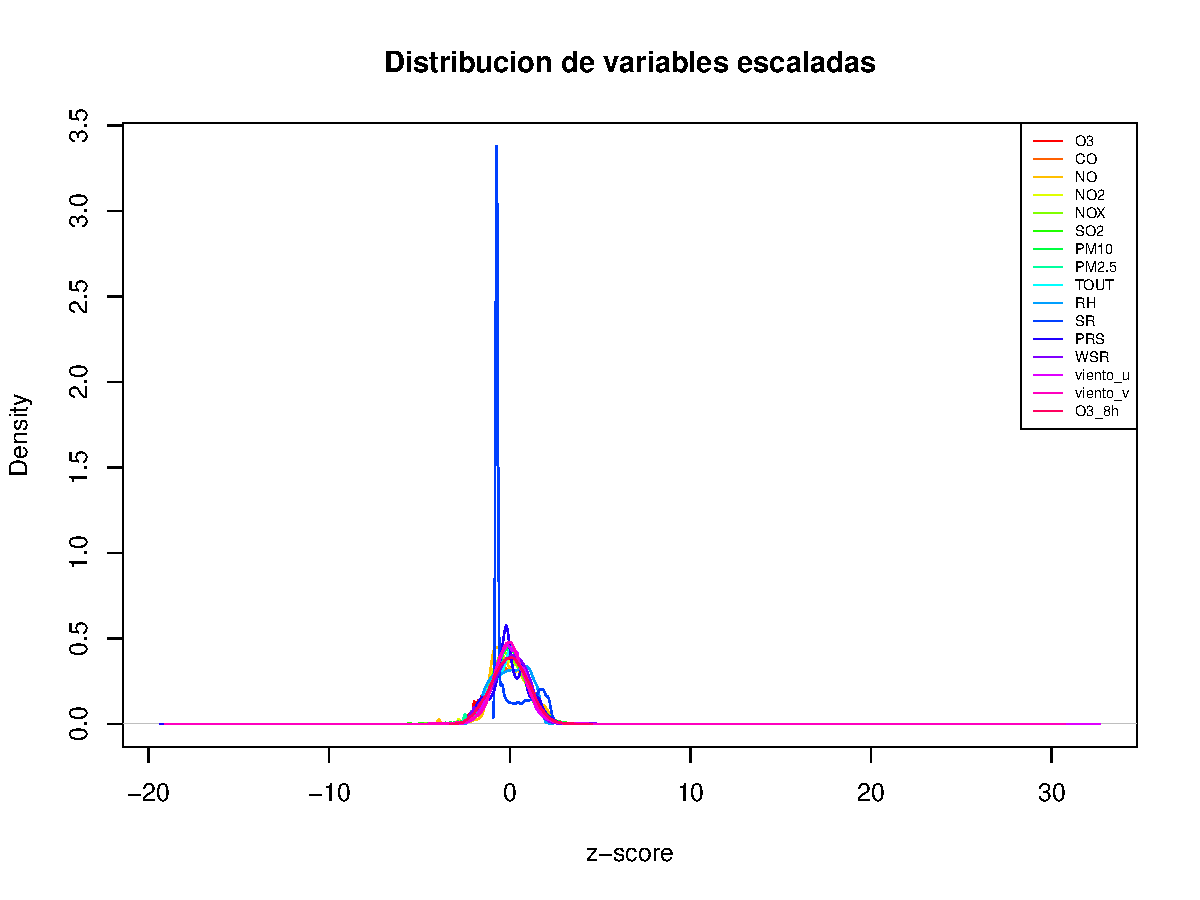
\includegraphics[width=\linewidth]{densidad_variables_escaladas.pdf}
  \caption{Distribución (densidad) de las variables cuantitativas tras la transformación Box-Cox y el escalamiento.}
  \label{fig:densidad-escaladas}
\end{figure}

El diccionario del conjunto transformado, con la descripción completa de cada
variable, su tratamiento y su sesgo antes y después, se documenta en el
\cref{sec:diccionario-transformado}.

      % \subsection

% 4. Análisis exploratorio
% Seccion 4 de la rubrica no la exige, pero el analisis exploratorio es lo
% que justifica el ACP y la eleccion del umbral. Aloja como \subsection a
% eda_cualitativas.tex. Las tablas exhaustivas de estadisticos viven en el
% diccionario (anexo); aqui solo lo que se interpreta.

\section{Análisis exploratorio}
\label{sec:eda}

\subsection{Variables cuantitativas}

\subsubsection{Cuartiles y límites de outliers}

Los cuartiles y límites de $1.5\times$IQR de las variables horarias se
reportan en sus unidades originales (\cref{tab:cuartiles-iqr}) y son los
mismos que usó la limpieza como criterio de outliers. \texttt{RAINF} y
\texttt{WDR} quedan fuera: \texttt{WDR} es circular y \texttt{RAINF} está
inflada de ceros, así que su IQR no es interpretable como límite
(\cref{sec:dic:meteorologicos}). Dos lecturas importan para lo que sigue: la
mediana de la componente zonal del viento es negativa, es decir, el viento
predominante entra del oriente (\cref{sec:contexto-estaciones}); y el límite
superior de \texttt{O3\_8h} (66.22 ppb) queda por encima del umbral de
51 ppb, de modo que la excedencia no es un outlier sino parte del rango
habitual de la variable.

\begin{table}[t]
  \centering
  \caption{Cuartiles y límites de outlier (criterio $1.5\times$IQR) de las
    variables cuantitativas horarias, en sus unidades originales.}
  \label{tab:cuartiles-iqr}
  \small
  \begin{tabular}{lrrrr}
    \toprule
    Variable & Q1 & Q3 & Lím. inf. & Lím. sup. \\
    \midrule
    \texttt{O3}       &    13.00 &    37.00 &  $-23.00$ &    73.00 \\
    \texttt{CO}       &     0.71 &     1.83 &   $-0.96$ &     3.50 \\
    \texttt{NO2}      &     6.90 &    19.70 &  $-12.30$ &    38.90 \\
    \texttt{NOX}      &    10.95 &    30.70 &  $-18.68$ &    60.33 \\
    \texttt{PM10}     &    35.00 &    74.00 &  $-23.50$ &   132.50 \\
    \texttt{PM2.5}    &    10.00 &    26.74 &  $-15.11$ &    51.85 \\
    \texttt{TOUT}     &    18.49 &    28.39 &      3.64 &    43.24 \\
    \texttt{PRS}      &   709.70 &   721.70 &    691.70 &   739.70 \\
    \texttt{WSR}      &     4.70 &    11.60 &   $-5.65$ &    21.95 \\
    \texttt{O3\_8h}   &    15.44 &    35.75 &  $-15.03$ &    66.22 \\
    \texttt{viento\_u}&  $-8.56$ &     0.21 &  $-21.73$ &    13.37 \\
    \texttt{viento\_v}&  $-3.38$ &     3.98 &  $-14.41$ &    15.01 \\
    \bottomrule
  \end{tabular}
\end{table}

La \cref{fig:boxplot-medidas} muestra la distribución de cada variable en
unidades originales. Todas las concentraciones de contaminantes presentan
cola derecha larga, con outliers que multiplican varias veces el tercer
cuartil; es la asimetría que motivó Box-Cox en \cref{sec:transformaciones}.
Las meteorológicas son más simétricas, salvo la velocidad del viento.

\begin{figure}[t]
    \centering
    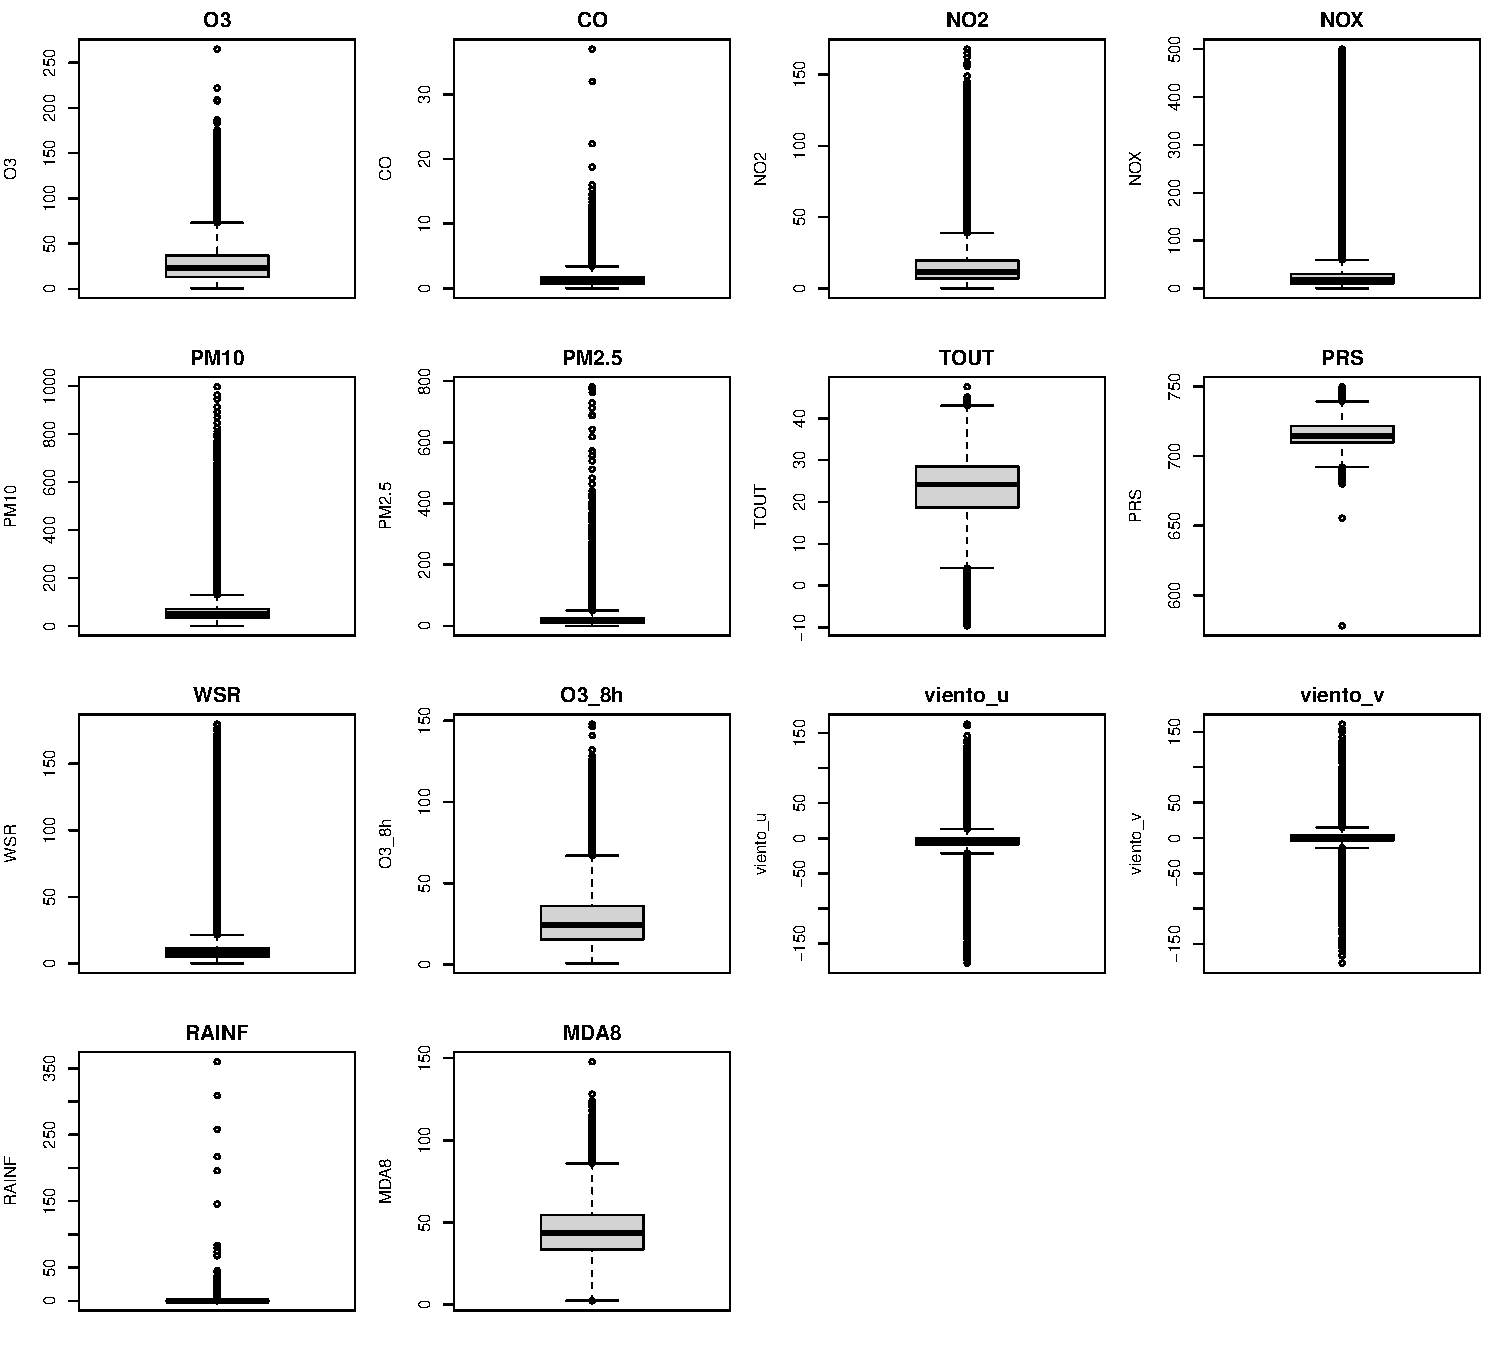
\includegraphics[width = \linewidth]{boxplots_medidas.pdf}
    \caption{Diagramas de caja de cada variable cuantitativa horaria, en
      unidades originales.}
    \label{fig:boxplot-medidas}
\end{figure}

\subsubsection{Correlación}

A resolución horaria y sobre la escala transformada, los pares más fuertes
son \texttt{NO2}--\texttt{NOX} ($r=0.89$), multicolinealidad esperada entre
precursores del mismo ciclo de reacción; \texttt{O3}--\texttt{O3\_8h}
($r=0.69$), por construcción; \texttt{PM10}--\texttt{PM2.5} ($r=0.62$),
material particulado de origen común; \texttt{O3}--\texttt{TOUT} ($r=0.52$)
y \texttt{O3}--\texttt{WSR} ($r=0.43$), consistentes con el mecanismo
fotoquímico; y \texttt{O3}--\texttt{NOX} ($r=-0.43$), que refleja el consumo
de \ce{O3} por titulación con \ce{NO} cerca de fuentes de tráfico.

El ACP corre sobre la tabla diaria y necesita su propia matriz: agregar a
día cambia el tamaño de muestra y, típicamente, sube la correlación al
cancelar ruido de medición. Se calcula sobre las 16 variables continuas del
conjunto diario transformado, en el subconjunto con las 16 simultáneamente
completas ($n=15{,}856$ de 26,691 días-estación, 59.4\,\%), la misma regla
de descarte por lista que usa el modelado y que garantiza una matriz
semidefinida positiva (\cref{fig:mapa-calor-diario}).

\begin{figure}[t]
    \centering
    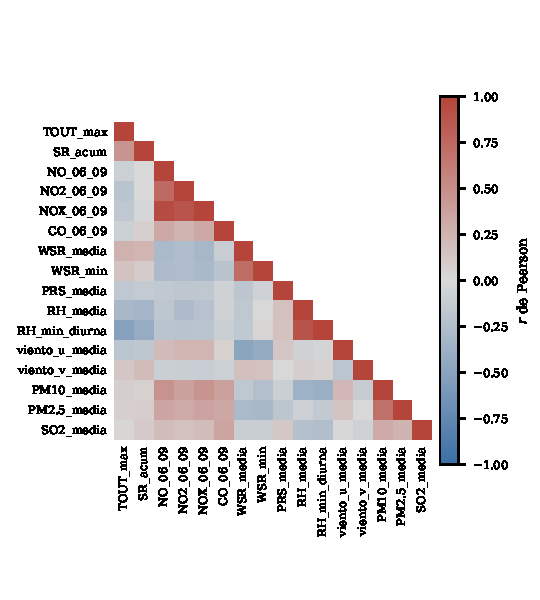
\includegraphics[width = \linewidth]{mapa_calor_correlacion_diario.pdf}
    \caption{Mapa de calor de correlación de Pearson entre las 16 variables
      continuas del conjunto diario transformado, $n=15{,}856$ días-estación
      completos.}
    \label{fig:mapa-calor-diario}
\end{figure}

De los pares horarios, tres tienen análogo directo en el conjunto diario:
\texttt{NO2}--\texttt{NOX} no cambia (0.89), \texttt{PM10}--\texttt{PM2.5}
sube a 0.70 y \texttt{viento\_u}--\texttt{WSR} sube en magnitud a $-0.48$.
El orden sí cambia: dominan \texttt{NO}--\texttt{NOX} ($r=0.95$) y
\texttt{RH\_media}--\texttt{RH\_min\_diurna} ($r=0.89$), inexistentes en el
mapa horario porque \texttt{NO} y \texttt{RH} no formaban parte de ese
conjunto. El primero es la redundancia definicional \texttt{NOX} $\approx$
\texttt{NO} + \texttt{NO2}; el segundo, y también
\texttt{WSR\_media}--\texttt{WSR\_min} ($r=0.71$), es la misma variable
resumida dos veces sobre ventanas distintas del día. Estas redundancias de
construcción son las que el análisis factorial (\cref{sec:analisis-factorial})
termina por expulsar.

Los diagnósticos previos al ACP confirman la multicolinealidad
(\cref{tab:diagnostico-pca}): el determinante es cercano a 0 y el número de
condición es alto. La prueba de esfericidad de Bartlett rechaza que la
matriz sea la identidad ($\chi^2(120)=169{,}140.7$, $p<0.001$), y el KMO
total libra el umbral convencional de 0.6; a nivel variable,
\texttt{RH\_media} (0.587), \texttt{PRS\_media} (0.589) y \texttt{TOUT\_max}
(0.596) quedan justo debajo sin arrastrar el total. Los cuatro diagnósticos
justifican aplicar ACP sobre los predictores diarios.

\begin{table}[t]
  \centering
  \caption{Diagnósticos previos al ACP sobre la matriz de correlación
    diaria ($n=15{,}856$, 16 variables).}
  \label{tab:diagnostico-pca}
  \small
  \begin{tabular}{lr}
    \toprule
    Diagnóstico          & Valor \\
    \midrule
    Determinante          & $2.32\times10^{-5}$ \\
    Número de condición   & 322.8 \\
    KMO total             & 0.660 \\
    \bottomrule
  \end{tabular}
\end{table}

\subsection{Variables cualitativas}
\label{sec:eda-cualitativas}

Las categóricas se reportan en dos bloques por unidad de análisis:
\texttt{periodo} y \texttt{llovio} solo existen a resolución horaria; las
indicadoras de excedencia derivan del MDA8 y solo existen a resolución
diaria. Mezclarlas replicaría cada valor diario 24 veces. Las bases son
$n = 640{,}583$ registros hora-estación y $n = 26{,}691$ día-estación.

\subsubsection{Distribución de frecuencia}

\Cref{tab:freq-horaria} reúne las variables horarias. Con 2025 completo las
cuatro temporadas quedan equilibradas (24.79\,\% a 25.16\,\%), de modo que
ningún contraste estacional es artefacto de la ventana de observación.
\texttt{periodo} es uniforme por construcción: cuatro bloques de 6 horas
sobre una rejilla horaria completa. \texttt{llovio} es la única horaria con
faltantes (19,360 registros, 3.02\,\%), que se conservan como categoría
propia en vez de asignarse a ``no llovió''; llueve en 1.49\,\% de las horas
con medición. \texttt{tipo\_dia} sustituye a la binaria de fin de semana
porque separa sábado de domingo, cuyos patrones vehiculares difieren, y
aísla los 71 días festivos del periodo.

\begin{table}[t]
  \centering
  \caption{Frecuencia absoluta y relativa de las variables cualitativas a
    resolución hora-estación ($n = 640{,}583$). Los porcentajes son sobre
    registros con dato válido.}
  \label{tab:freq-horaria}
  \small
  \begin{tabular}{llrr}
    \toprule
    Variable & Nivel & Frecuencia & \% \\
    \midrule
    \multirow{4}{*}{\texttt{temporada}}
                                  & Invierno  &   158,783 &  24.79 \\
                                  & Primavera &   161,184 &  25.16 \\
                                  & Verano    &   161,184 &  25.16 \\
                                  & Otoño     &   159,432 &  24.89 \\
    \midrule
    \multirow{4}{*}{\texttt{periodo}}
                                  & Madrugada &   160,145 &  25.00 \\
                                  & Mañana    &   160,146 &  25.00 \\
                                  & Tarde     &   160,146 &  25.00 \\
                                  & Noche     &   160,146 &  25.00 \\
    \midrule
    \multirow{4}{*}{\texttt{tipo\_dia}}
                                  & Laborable &   434,879 &  67.89 \\
                                  & Sábado    &    88,392 &  13.80 \\
                                  & Domingo   &    88,728 &  13.85 \\
                                  & Festivo   &    28,584 &   4.46 \\
    \midrule
    \multirow{3}{*}{\texttt{llovio}}
                                  & No (0)    &   611,952 &  98.51 \\
                                  & Sí (1)    &     9,271 &   1.49 \\
                                  & Sin dato  &    19,360 &    --- \\
    \bottomrule
  \end{tabular}
\end{table}

\Cref{tab:freq-diaria} presenta el bloque diario. Las tres indicadoras de
MDA8 comparten los mismos 1,591 registros sin dato (5.96\,\%), los
días-estación cuyo MDA8 no alcanzó la completitud de 18 de 24 ventanas;
\texttt{excede\_1h} no los comparte porque se calcula sobre el máximo
horario.

\begin{table}[t]
  \centering
  \caption{Frecuencia absoluta y relativa de las indicadoras de excedencia a
    resolución día-estación ($n = 26{,}691$; válidos $= 25{,}100$ para las
    indicadoras de MDA8).}
  \label{tab:freq-diaria}
  \small
  \begin{tabular}{llrr}
    \toprule
    Variable & Nivel & Frecuencia & \% \\
    \midrule
    \multirow{3}{*}{\texttt{excede\_anio\_1} (65 ppb)}
                                        & No excede &  22,275 &  88.75 \\
                                        & Excede    &   2,825 &  11.25 \\
                                        & Sin dato  &   1,591 &    --- \\
    \midrule
    \multirow{3}{*}{\texttt{excede\_anio\_3} (60 ppb)}
                                        & No excede &  20,864 &  83.12 \\
                                        & Excede    &   4,236 &  16.88 \\
                                        & Sin dato  &   1,591 &    --- \\
    \midrule
    \multirow{3}{*}{\texttt{excede\_anio\_5} (51 ppb)}
                                        & No excede &  17,079 &  68.04 \\
                                        & Excede    &   8,021 &  31.96 \\
                                        & Sin dato  &   1,591 &    --- \\
    \midrule
    \multirow{2}{*}{\texttt{excede\_1h} (90 ppb)}
                                        & No excede &  24,497 &  91.78 \\
                                        & Excede    &   2,194 &   8.22 \\
    \bottomrule
  \end{tabular}
\end{table}

\subsubsection{La estación de monitoreo}

Catorce de las 15 estaciones registran 43,824 observaciones cada una, la
rejilla horaria completa de 2021-01-01 a 2025-12-31; \texttt{NO3} registra
27,047 porque inicia operación el 1 de diciembre de 2022. La diferencia es de
cobertura, no de calidad: dentro de su ventana \texttt{NO3} también tiene
rejilla completa y su porcentaje de horas con \ce{O3} medido está dentro del
rango del resto de la red. \texttt{periodo}, la única
ordinal, tiene mediana \texttt{tarde} sobre las 611,601 horas con \ce{O3}
medido, porque los faltantes se concentran de noche.

\subsubsection{Balance de clases}

\Cref{fig:eda-cual-excedencias} visualiza el balance de las tres indicadoras
de MDA8. Al umbral vigente de 65 ppb las excedencias son 11.25\,\% de los
días-estación válidos: un clasificador que prediga siempre la clase
mayoritaria alcanza 88.75\,\% de aciertos sin capturar el fenómeno, y la
exactitud queda descartada como métrica en favor de sensibilidad,
especificidad y área bajo la curva ROC. El umbral de 51 ppb, con
31.96\,\%, ofrece un balance sustancialmente mejor y es el escenario
principal de modelado.

\begin{figure}[t]
  \centering
  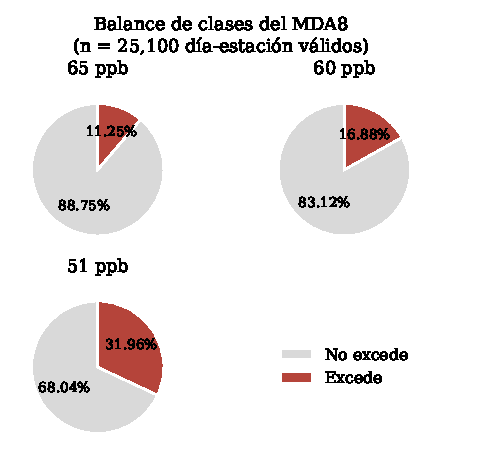
\includegraphics[width=\linewidth]{eda_cual_excedencias.pdf}
  \caption{Balance de clases de las indicadoras de excedencia del MDA8 para los
    tres umbrales de cumplimiento gradual de la NOM-020-SSA1-2021
    (\cref{tab:nom-limites}).}
  \label{fig:eda-cual-excedencias}
\end{figure}
      % \subsection

% 5. Modelación y validación
% Seccion 5 de la rubrica: modelacion y validacion. Solo abre la seccion y
% fija lo comun a todas las tecnicas (particion, regla de fuga). Cada tecnica
% es una \subsection en su propio archivo.

\section{Modelación y validación}
\label{sec:modelacion}

Todas las técnicas comparten la misma partición temporal: los años
2021--2024 se destinan al ajuste y 2025 completo a la validación. La regla
es estricta: ningún procedimiento ve 2025 durante el ajuste, incluidos el
ACP y el AF, cuyos ejes se estiman sobre 2021--2024 y se aplican a 2025 con
los pesos de entrenamiento; de otro modo la información de la partición de
validación se filtraría a las coordenadas que consumen los clasificadores.
La única fuga que persiste es la del parámetro $\lambda$ de Box-Cox,
estimado sobre el periodo completo en \cref{sec:transformaciones}; se
declara porque revertirla exigiría rehacer el conjunto transformado.

La validación tiene una particularidad que atraviesa todos los resultados:
2025 es el año de ozono más alto de la serie, con 44.0\,\% de excedencia
día-estación contra 29.4\,\% del ajuste, en las cuatro temporadas. Es un
efecto de año, no de calendario, y cada técnica lo retoma donde le afecta.

Las cinco técnicas se presentan en el orden en que cada una alimenta a la
siguiente: el ACP (\cref{sec:pca}) y el AF (\cref{sec:analisis-factorial})
reducen los 16 predictores a tres ejes; la caracterización como serie de
tiempo (\cref{sec:serie-tiempo}) establece la dependencia temporal de esos
ejes; la regresión logística y el discriminante
(\cref{sec:clasificacion_tecs}) clasifican el día-estación; y el modelo
autorregresivo (\cref{sec:autorregresivo}) incorpora la dependencia temporal
a la clasificación.
            % \section + partición común
\subsection{Componentes principales}\label{sec:pca}

Los predictores diarios no son coordenadas independientes: \texttt{NO2} y
\texttt{NOX} comparten la mayor parte de su variación, y otro tanto ocurre entre
\texttt{PM10} y \texttt{PM2.5}. El análisis de componentes principales no
persigue aquí un objetivo propio, sino sustituir ese bloque correlacionado por
un conjunto de ejes ortogonales que el modelo de clasificación pueda emplear sin
inflar los errores estándar de sus coeficientes.

\subsubsection{Bloque de predictores}

Entran las variables continuas de precursores y meteorología. Las indicadoras de
zona, \texttt{tipo\_dia}, \texttt{temporada} y \texttt{festivo} quedan fuera,
porque una columna binaria eleva de forma artificial la varianza explicada; se
incorporan directamente a la etapa de modelado. También se excluyen \ce{MDA8},
\texttt{O3\_max\_1h} y las indicadoras de excedencia, que constituyen la
respuesta y cuya inclusión como predictores sería fuga de información.

\texttt{PM2.5} se retira del bloque. La estación \texttt{NE3} no registra un
solo valor de esa variable y \texttt{NO3} registra 12.5\,\%, de modo que exigir
observaciones completas no descarta días aislados sino estaciones enteras: la
retención de la zona Noroeste caería de 60.5\,\% a 44.0\,\%, justamente la zona
de mayor tasa de excedencia. La dimensión de aerosoles permanece representada
por \texttt{PM10}. El bloque final reúne 15 predictores.

\subsubsection{Ajuste y criterio de retención}

La descomposición se ajusta sobre la matriz de correlación de los años 2021 a
2024 y se aplica al año 2025 mediante los mismos vectores propios y momentos de
entrenamiento; ajustarla sobre el periodo completo transferiría información del
conjunto de validación a la construcción de los ejes. El ajuste emplea 16{,}008
observaciones y la proyección de validación, 1{,}340.

El criterio de retención se fijó antes de ejecutar el análisis: método del codo
sobre el gráfico de sedimentación, presentado en \cref{fig:pca-scree}. La
curvatura del perfil de valores propios alcanza su máximo en la tercera
componente, con 1.13 frente a 0.26 en la cuarta, y las caídas sucesivas
confirman la lectura: el tramo pronunciado termina en la tercera componente y a
partir de ahí la pendiente se aplana. Se retienen tres componentes, que reúnen
55.9\,\% de la varianza.

El criterio de Kaiser retendría cinco componentes y 71.0\,\% de la varianza. Se
reporta como contraste, sin modificar la decisión: el umbral $\lambda > 1$ es
fijo y no considera la forma del perfil. Una lectura alternativa del codo, la de
máxima distancia a la recta que une los extremos, sitúa el punto en la cuarta
componente, si bien con un margen de 3\,\% sobre la tercera.

\begin{figure}[t]
  \centering
  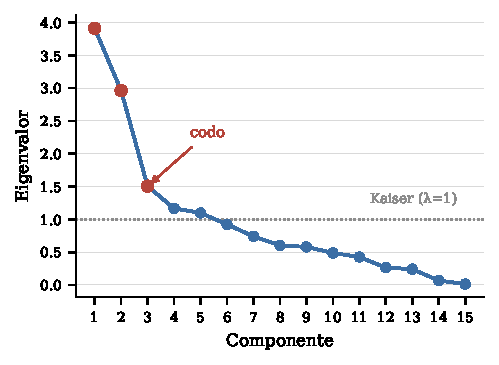
\includegraphics[width=\linewidth]{pca_scree.pdf}
  \caption{Gráfico de sedimentación de los 15 predictores. El codo por
    curvatura se ubica en la tercera componente; la línea punteada marca el
    umbral de Kaiser.}
  \label{fig:pca-scree}
\end{figure}

\subsubsection{Interpretación de los ejes}

\cref{tab:pca-cargas} reúne las cargas dominantes de cada componente retenida.
Las tres admiten lectura física, lo que permite interpretar después los
coeficientes del modelo de clasificación en términos de condiciones
atmosféricas y no de componentes numeradas.

\begin{table}[h]
  \centering
  \caption{Cargas dominantes de las componentes retenidas, con la varianza que
    explica cada una.}
  \label{tab:pca-cargas}
  \begin{tabular}{lr}
    \toprule
    Componente y variable & Carga \\
    \midrule
    \multicolumn{2}{l}{\emph{Carga primaria de combustión} (26.1\,\%)} \\
    \quad \texttt{NOX}      & 0.88 \\
    \quad \texttt{NO}       & 0.82 \\
    \quad \texttt{NO2}      & 0.81 \\
    \quad \texttt{PM10}     & 0.66 \\
    \quad \texttt{WSR\_min} & $-0.48$ \\
    \midrule
    \multicolumn{2}{l}{\emph{Forzamiento fotoquímico} (19.8\,\%)} \\
    \quad \texttt{RH\_min\_diurna} & $-0.77$ \\
    \quad \texttt{TOUT\_max}       & 0.72 \\
    \quad \texttt{RH\_media}       & $-0.70$ \\
    \quad \texttt{SR\_acum}        & 0.65 \\
    \quad \texttt{WSR\_media}      & 0.60 \\
    \midrule
    \multicolumn{2}{l}{\emph{Estancamiento atmosférico} (10.0\,\%)} \\
    \quad \texttt{WSR\_min}        & $-0.50$ \\
    \quad \texttt{viento\_u\_media} & 0.48 \\
    \quad \texttt{WSR\_media}      & $-0.41$ \\
    \quad \texttt{PRS\_media}      & 0.39 \\
    \quad \texttt{RH\_min\_diurna} & $-0.37$ \\
    \bottomrule
  \end{tabular}
\end{table}

La primera componente agrupa los precursores de emisión vehicular en la ventana
matutina, acompañados de material particulado y de velocidad de viento con signo
negativo: describe la acumulación de carga primaria cuando el aire no la
dispersa. La segunda opone temperatura máxima y radiación acumulada a humedad
relativa, la firma de un día caluroso, despejado y seco. La tercera combina
viento débil con presión elevada, el patrón anticiclónico.

Este último eje merece una precisión metodológica. La combinación de viento
débil y presión alta no se construyó como índice para después presentarla como
resultado: emerge de la descomposición, que agrupa esas variables por su
covariación observada. \cref{fig:pca-biplot} muestra la estructura en los dos
planos definidos por la primera componente.

\begin{figure*}[t]
  \centering
  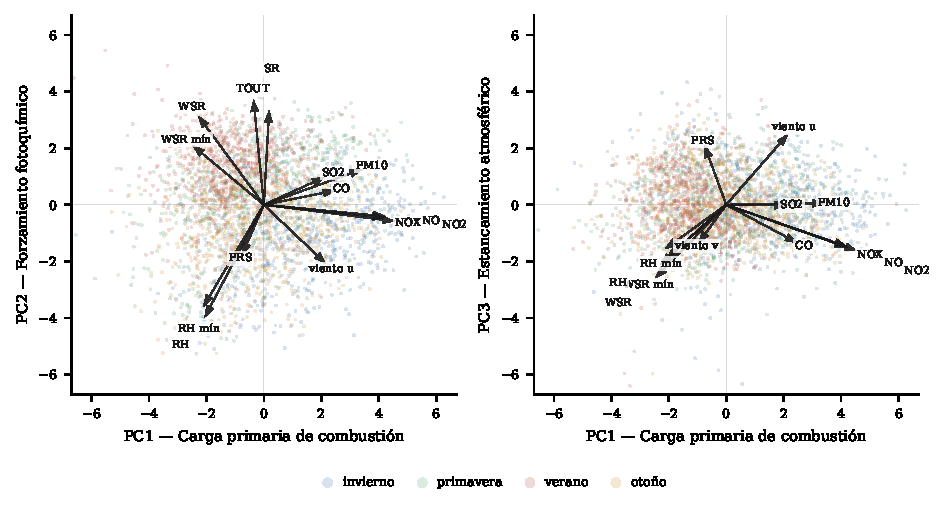
\includegraphics[width=\linewidth]{pca_biplot.pdf}
  \caption{Biplot de las componentes retenidas. Los puntos corresponden a una
    submuestra de 3{,}000 observaciones de entrenamiento, coloreadas por
    temporada; las flechas representan las cargas escaladas al marco del
    gráfico.}
  \label{fig:pca-biplot}
\end{figure*}

Los nombres describen la composición de cada eje y no atribuyen un mecanismo de
formación. El conjunto no incluye mediciones de compuestos orgánicos volátiles,
por lo que las componentes se describen como consistentes con procesos de
combustión, fotoquímica y estancamiento, sin sustentar afirmación alguna sobre
el régimen que limita la producción de ozono.

Queda una limitación del procedimiento. Los parámetros de la transformación
Box-Cox descrita en \cref{sec:transformaciones} se estimaron sobre el periodo
completo, de modo que la forma marginal de cada variable incorpora información
del año 2025. El efecto no alcanza a la variable respuesta ni a la construcción
de los ejes, que se ajustan únicamente con los años de entrenamiento.
                   % \subsection
\subsection{Análisis factorial exploratorio}
\label{sec:analisis-factorial}

El análisis factorial complementa al ACP (\cref{sec:pca}) al separar
la varianza compartida entre variables de la específica de cada una.
Para cada variable
estandarizada se plantea
\begin{equation}
  z_j=\sum_{k=1}^{3}\lambda_{jk}f_k+\varepsilon_j,
  \qquad h_j^2=\sum_{k=1}^{3}\lambda_{jk}^2.
  \label{eq:af-modelo}
\end{equation}
Los $f_k$ son factores latentes y las cargas $\lambda_{jk}$ indican
la magnitud y el sentido de su asociación con cada variable. Con
factores ortogonales de varianza unitaria, la comunalidad $h_j^2$ es
la proporción de varianza explicada; la unicidad $1-h_j^2$ recoge
la parte específica y el error.

\paragraph{Adecuación y extracción}
El diagnóstico inicial utiliza 15 predictores y 16,028 observaciones
completas de 2021--2024. Bartlett
rechaza la ausencia de correlaciones ($p<0.001$), aunque la dependencia
temporal y espacial limita esta prueba. El KMO inicial de 0.647
indica adecuación mediocre. Se retira \texttt{NOX\_06\_09} por su
redundancia con NO y NO2 (VIF de 45.73). Sobre las 14 variables
restantes, MAP de Velicer sugiere tres factores, frente a siete del
análisis paralelo; se adopta MAP por parsimonia, conservando esta
discrepancia como limitación.

La extracción por ejes principales iterados produce una comunalidad
inadmisible de 1.093 para \texttt{RH\_min\_diurna}; se elimina esta
variable y se conserva la humedad media. El bloque final de 13
predictores alcanza un KMO de 0.677 y un VIF máximo de 2.54, sin
comunalidades superiores a uno. Se mantienen tres factores y se
aplica varimax para facilitar su interpretación mediante ejes
ortogonales (\cref{fig:af-diagrama}).

\begin{figure}[t]
  \centering
  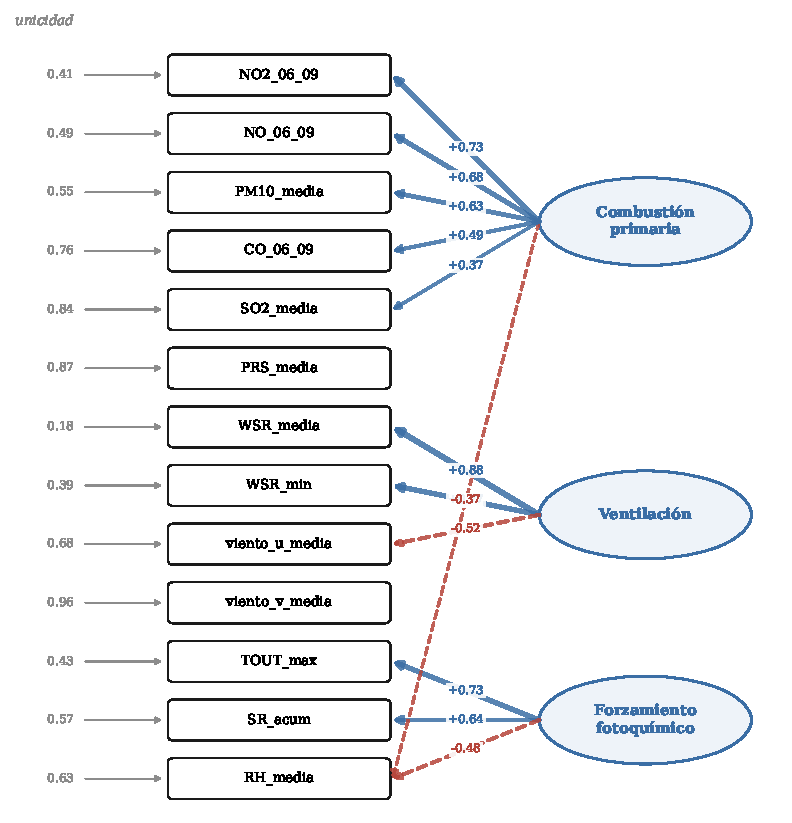
\includegraphics[width=0.92\linewidth]{af_diagrama_cargas.pdf}
  \caption{Cargas varimax con $|\lambda|\geq0.30$. Flechas sólidas:
  asociaciones positivas; discontinuas: negativas. Los valores grises
  indican unicidades.}
  \label{fig:af-diagrama}
\end{figure}

\paragraph{Interpretación}
Los factores explican el 40.3\,\% de la varianza total de los 13
predictores. \emph{Combustión primaria} (15.7\,\%) agrupa NO2 (0.74), NO
(0.68), PM10 (0.63), CO (0.49) y SO2. \emph{Ventilación} (14.5\,\%) reúne
la velocidad media y mínima del viento, con cargas de 0.88 y 0.77, y la
componente zonal ($-0.52$). \emph{Forzamiento fotoquímico} (10.1\,\%)
combina temperatura máxima (0.72), radiación acumulada (0.63) y humedad
media ($-0.48$): días
cálidos, soleados y secos. La presión tiene comunalidad de apenas
0.13, por lo que el nombre ventilación resulta más preciso que
atribuir al factor un mecanismo anticiclónico.

Tres decisiones que se probaron y se descartaron en el camino ---el análisis paralelo de Horn, la extracción por máxima verosimilitud y la rotación oblicua--- se documentan en \cref{sec:tecnicas-descartadas}.

\paragraph{Ajuste y alcance}
El residuo cuadrático medio de las correlaciones reconstruidas
(RMSR) es 0.0555; 26 de 78 pares conservan residuos absolutos mayores
que 0.05. El ajuste es razonable, pero parcial. Los puntajes de
Bartlett, aplicados a 2025 con pesos de entrenamiento, tienen VIF
cercanos a 1.01 y correlación absoluta máxima de 0.097. Por eso son
los predictores de los modelos de \cref{sec:clasificacion_tecs}, en lugar
de las puntuaciones del ACP, cuyo contraste se reporta ahí.

Los tres factores reaparecen en 2025 con congruencia de Tucker de
0.973 para combustión, 0.939 para ventilación y 0.924 para fotoquímica:
la estructura es estable fuera del periodo de ajuste. La determinación de
los puntajes (correlación entre puntaje y factor) es 0.880, 0.918 y 0.833;
el forzamiento fotoquímico comparte 69\,\% de su varianza con el factor
que representa, y el resto es error de estimación. Persisten el KMO
mediocre y la transformación Box--Cox estimada sobre todo el periodo. Los factores describen asociaciones; sin mediciones de
compuestos orgánicos volátiles no permiten establecer mecanismos
de formación de ozono.
    % \subsection
\subsection{Serie de tiempo de los puntajes factoriales y la excedencia}\label{sec:serie-tiempo}

Los tres puntajes factoriales de \cref{sec:analisis-factorial} y \texttt{excede\_anio\_5}
(\cref{sec:obj:objetivo}) se caracterizan aquí en el tiempo: no se reabre su
origen ni su validez, ya establecidos, sino su comportamiento como series.

\subsubsection{De día-estación a área metropolitana}

Antes de aplicar cualquier descomposición de serie de tiempo hace falta una
serie sin huecos, y el panel día-estación no lo es. Solo 2 de las 15
estaciones (\texttt{CE}, \texttt{SE3}) superan 85\,\% de cobertura de
día-estación válido sobre el calendario 2021--2025, y la peor,
\texttt{NO3}, llega a 25\,\%; la cobertura global es 68.0\,\%. Filtrar a las estaciones de mejor
cobertura no resuelve el problema, lo esconde en las tres que sobreviven al
corte.

La alternativa es agregar las 15 estaciones a un valor diario de área
metropolitana, lo que solo es razonable si las estaciones no son
independientes entre sí el mismo día. La correlación transversal (Pearson,
estación contra estación, mismo día) va de una media de 0.50 en ventilación a
0.85 en forzamiento fotoquímico, con un mínimo apenas negativo únicamente en
ventilación. Es coherente con la física: la temperatura y la radiación solar
son fenómenos de escala regional, y el viento depende de la topografía local
del valle. Esta correlación es también la violación de independencia más
grande del conjunto de datos, relevante para cualquier modelo que trate cada
fila día-estación como una observación --- incluida la limitación de
autocorrelación ya declarada en \cref{sec:limitaciones-clasificacion}.

Con la cobertura insuficiente por estación y la correlación transversal alta,
se agrega a nivel área metropolitana promediando las estaciones que reportan
cada día. El promedio recupera 99.94\,\% de cobertura del calendario diario;
un único día, el 2021-02-16, se queda sin ninguna estación y se imputa por
interpolación lineal --- solo porque la descomposición MSTL exige una serie
sin huecos, no porque el hueco deje de existir.

\subsubsection{Descomposición MSTL}

Se ajusta MSTL con periodos semanal (7) y anual (365, no 365.25: MSTL exige
periodos enteros y el corrimiento acumulado en 4.5 años es de un día,
despreciable) a las cuatro series de área metropolitana. El ciclo semanal es
más fuerte en combustión primaria --- el patrón entre semana / fin de semana
del tráfico y la actividad industrial --- y más débil en la fracción de
estaciones que excede el umbral, que diluye ese patrón al depender de varios
factores a la vez.

\subsubsection{Autocorrelación residual}

La prueba de Ljung-Box en los rezagos 7, 14 y 30 rechaza con $p<0.001$ en las
cuatro series, en ambas versiones (cruda y residual de MSTL) --- el mismo
problema que \cref{sec:analisis-factorial} documentó para Bartlett: con $n=1{,}826$
observaciones diarias, el estadístico crece con $n$ y rechaza cualquier
autocorrelación no trivial, incluida la del residual donde la estacionalidad
ya se removió. La prueba no discrimina; la magnitud de la ACF sí
(\cref{fig:acf-excedencia}).

\begin{figure}[t]
  \centering
  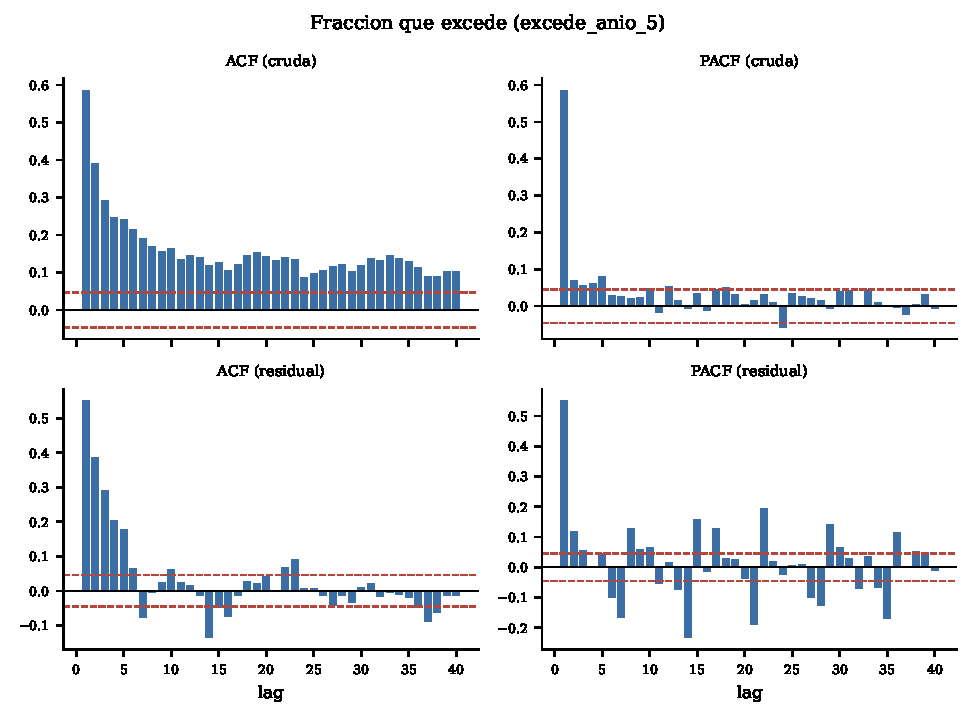
\includegraphics[width=\linewidth]{acf_pacf_frac_excede_anio_5.pdf}
  \caption{ACF y PACF hasta el rezago 40 de la fracción que excede: serie
    cruda (arriba) contra residual de la descomposición MSTL (abajo), con
    banda $\pm 1.96/\sqrt{n}$.}
  \label{fig:acf-excedencia}
\end{figure}

Tras MSTL, la autocorrelación en el rezago 7 cae de 0.19--0.45 a valores
entre $-0.15$ y 0.05 en las cuatro series --- la estacionalidad semanal
prácticamente desaparece. La del rezago 1, en cambio, se mantiene entre 0.49 y
0.71 en el residual de las cuatro series. Esa persistencia de un día para
otro no es estacionalidad: es autocorrelación genuina de corto plazo, que
MSTL no está diseñado para remover. Cuantifica, con una serie continua y sin
huecos, la misma dependencia temporal que \cref{sec:limitaciones-clasificacion}
señaló como razón de que los errores estándar del modelo logístico sean
optimistas.

Dos consecuencias pasan al modelo autorregresivo de
\cref{sec:autorregresivo}: los rezagos deben calcularse sobre la serie de
área metropolitana reindexada a calendario diario regular, nunca sobre la
tabla día-estación, donde la fila anterior puede estar a una semana de
distancia; y la dependencia de un día para otro es genuina, no un artefacto
de estacionalidad, así que un modelo que la ignore deja estructura en los
residuales.
% \subsection
% Tecnicas de dependencia sobre el dia-estacion. Predictores: los tres
% puntajes factoriales de analisis_factorial.tex (reescalados a varianza
% unitaria con los momentos de entrenamiento) mas 12 indicadoras. Las cifras
% vienen de docs/analisis_discriminante.pdf con el 2025 completo.

\subsection{Clasificación: regresión logística y análisis discriminante}
\label{sec:clasificacion_tecs}

Los puntajes factoriales de \cref{sec:analisis-factorial} se unen por
estación y fecha con las variables categóricas del día-estación y con la
respuesta \texttt{excede\_anio\_5}. Los puntajes no tienen varianza unitaria
(desviaciones de 1.14, 1.10 y 1.21 en el ajuste), de modo que se reescalan
con la media y la desviación estándar de 2021--2024, nunca con las de 2025;
así cada razón de momios se lee por desviación estándar del factor y las
tres son comparables entre sí. Las categóricas \texttt{zona},
\texttt{tipo\_dia} y \texttt{temporada} entran como 12 indicadoras contra
los niveles de referencia Noreste, día laborable e invierno. La matriz de
diseño tiene 15 predictores; 16,058 filas entran al ajuste y 2,978 a la
validación.

\subsubsection{Regresión logística}\label{sec:reg_log}

El modelo se ajusta únicamente sobre 2021--2024. Las razones de momios se
reportan en la \cref{tab:momios-log}; ningún intervalo de los tres factores
cruza el 1. El forzamiento fotoquímico tiene el efecto mayor: una desviación
estándar adicional multiplica los momios de excedencia por 2.78, contra 1.92
de la combustión primaria. La lectura es química: los precursores son
necesarios pero la velocidad y el volumen de las reacciones que producen
ozono dependen de la temperatura y la radiación, por lo que la condición
fotoquímica pesa más que la disponibilidad de ingredientes. La ventilación
es el único factor protector (0.90): el viento dispersa.

\begin{table}[t]
  \centering
  \caption{Razones de momios del modelo logístico (\texttt{exp} del
    coeficiente) con intervalo del 95\,\% bajo independencia. Los factores se
    interpretan por desviación estándar; las indicadoras, contra su nivel de
    referencia: Noreste (zona), día laborable (\texttt{tipo\_dia}) e
    invierno (\texttt{temporada}). Todos los coeficientes son significativos
    ($p<0.001$) salvo \texttt{tipo\_dia\_sabado} ($p=0.04$) y
    \texttt{tipo\_dia\_festivo} ($p=0.13$).}
  \label{tab:momios-log}
  \small
  \begin{tabular}{lrc}
    \toprule
    Variable & Momios & IC 95\,\% \\
    \midrule
    Combustión primaria     & 1.92 & [1.82, 2.02] \\
    Ventilación             & 0.90 & [0.86, 0.95] \\
    Forzamiento fotoquímico & 2.78 & [2.62, 2.94] \\
    \midrule
    \texttt{zona\_Centro}    & 2.74 & [2.32, 3.22] \\
    \texttt{zona\_Noroeste}  & 3.84 & [3.32, 4.43] \\
    \texttt{zona\_Norte}     & 1.76 & [1.50, 2.06] \\
    \texttt{zona\_Sur}       & 2.90 & [2.44, 3.44] \\
    \texttt{zona\_Sureste}   & 1.82 & [1.59, 2.09] \\
    \texttt{zona\_Suroeste}  & 3.48 & [3.02, 4.01] \\
    \midrule
    \texttt{tipo\_dia\_sabado}  & 1.13 & [1.01, 1.27] \\
    \texttt{tipo\_dia\_domingo} & 1.43 & [1.27, 1.62] \\
    \texttt{tipo\_dia\_festivo} & 1.17 & [0.95, 1.44] \\
    \midrule
    \texttt{temporada\_primavera} & 3.54 & [3.08, 4.08] \\
    \texttt{temporada\_verano}    & 1.54 & [1.31, 1.83] \\
    \texttt{temporada\_otono}     & 3.04 & [2.66, 3.49] \\
    \bottomrule
  \end{tabular}
\end{table}

Las zonas con mayores momios son Noroeste (3.84) y Suroeste (3.48): a igual
meteorología y calendario, el poniente de la ciudad casi cuadruplica los
momios del Noreste, el ordenamiento espacial que
\cref{sec:contexto-estaciones} anticipó. La primavera (3.54) y el otoño
(3.04) triplican los momios del invierno, que con menor temperatura y
radiación frena las reacciones fotoquímicas aunque los precursores estén
presentes; el verano queda en 1.54. El calendario laboral apenas influye:
solo el domingo (1.43) tiene un efecto claro.

\paragraph{Errores estándar bajo dependencia.} Las 15 estaciones de un
mismo día comparten el clima y los días consecutivos se parecen, por lo que
los errores estándar bajo independencia son optimistas. Se corrigen con el
estimador sandwich agrupado por día (1,460 conglomerados): se inflan entre
1.5 y 2.5 veces, más en las indicadoras de calendario, constantes dentro de
un día, y nada en las de zona, que varían dentro de él. Los intervalos
corregidos de los tres factores son casi el doble de anchos y siguen sin
cruzar el 1 (\cref{fig:momios-corregido}): ventilación $[0.84, 0.97]$,
forzamiento fotoquímico $[2.48, 3.10]$. El único término que pierde
significancia al 5\,\% es el sábado. Agrupar además por estación no es
confiable con 15 conglomerados, pero deja claro que los siete contrastes de
zona descansan en 15 unidades, no en 16,058 filas.

\begin{figure}[t]
  \centering
  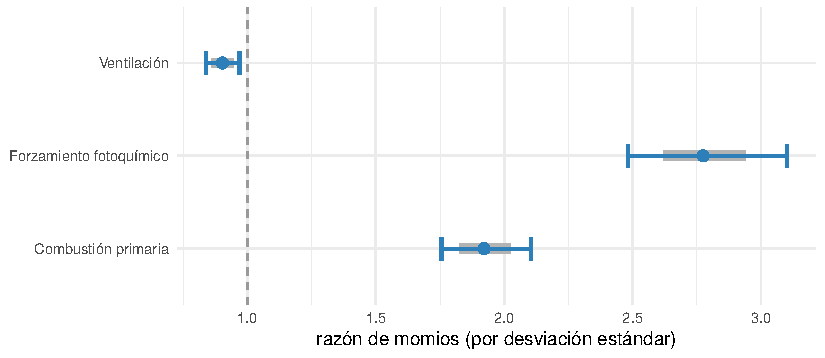
\includegraphics[width=\linewidth]{momios_ic_corregido.pdf}
  \caption{Razones de momios de los factores con intervalos del 95\,\% bajo
    independencia (gris) y agrupando por día (color). Los intervalos
    corregidos son más anchos y ninguno cruza el 1.}
  \label{fig:momios-corregido}
\end{figure}

\paragraph{Evaluación y validación.} La evaluación se realiza sobre 2025,
no visto durante el ajuste, con AUC, sensibilidad y especificidad; la
exactitud se descarta porque la tasa base de excedencia en validación es
43.97\,\%. El modelo alcanza un AUC de 0.850 (\cref{fig:roc-modelos}), por
encima del criterio de logro de 0.75. El umbral se elige por el índice de
Youden sobre el ajuste y resulta en 0.282; a ese umbral la sensibilidad es
0.698 y la especificidad 0.853 (panel izquierdo de la \cref{fig:matrices}).
Un umbral de 0.5 ilustra por qué la exactitud no sirve como criterio: la
especificidad sube a 0.964, pero la sensibilidad cae a 0.326, es decir, el
modelo deja de detectar dos de cada tres excedencias reales.

\subsubsection{Análisis discriminante lineal}\label{sec:lda}

La segunda técnica se ajusta sobre la misma matriz de diseño, la misma
respuesta y la misma partición. El contraste es deliberado: el discriminante
supone normalidad multivariada dentro de cada clase y homocedasticidad entre
clases, supuestos que la logística no requiere.

\paragraph{Verificación de supuestos.} Los puntajes factoriales son
combinaciones lineales de predictores con $|\text{sesgo}|<0.5$ tras Box-Cox.
Sobre los puntajes de entrenamiento separados por clase, los seis
coeficientes de sesgo quedan entre $-0.091$ y 0.489, de modo que la
aproximación a la normalidad se sostiene. La homocedasticidad no: no se
aplica la prueba M de Box, que con más de 15,000 observaciones rechaza
diferencias arbitrariamente pequeñas, sino la comparación directa de las
matrices de covarianza por clase. Los días de excedencia son menos dispersos
que los de no excedencia en los tres factores, con razones de desviación
estándar de 0.894, 0.888 y 0.742, y la varianza generalizada baja de 1.081 a
0.346; la discrepancia se concentra en el eje fotoquímico. Un segundo desvío
afecta a las 12 indicadoras binarias, que no son normales bajo ninguna
transformación. El discriminante lineal tolera ambos desvíos en la práctica,
y esa tolerancia se verifica empíricamente en \cref{sec:comparacion}.

\paragraph{Ajuste y evaluación.} Las probabilidades previas se fijan en las
proporciones observadas en el ajuste (0.706 y 0.294) porque la tasa base es
información del problema. Con dos clases hay una sola función
discriminante, y el orden y el signo de sus coeficientes reproducen los de
la \cref{tab:momios-log}: el forzamiento fotoquímico
(0.795) domina sobre la combustión primaria (0.506), la ventilación va en
contra ($-0.109$), el Noroeste y el Suroeste son las zonas de mayor riesgo y
la primavera (1.054) y el otoño (0.772) pesan más que el verano (0.176).
Los coeficientes indican la dirección de máxima separación entre clases; no
son razones de momios. La evaluación usa la
probabilidad posterior de excedencia como puntaje continuo, para que la ROC
sea comparable con la logística. El discriminante alcanza un AUC de 0.846;
al umbral de Youden (0.249) la sensibilidad es 0.758 y la especificidad
0.788 (panel derecho de la \cref{fig:matrices}).

\subsubsection{Comparación de los dos modelos}\label{sec:comparacion}

Las dos técnicas son prácticamente equivalentes sobre estos datos: los AUC
difieren en tres milésimas (0.850 contra 0.846), los puntajes correlacionan
a 0.996 y las clasificaciones coinciden en 93.8\,\% de los días-estación de
validación. La prueba de DeLong para curvas ROC correlacionadas sí detecta
la diferencia ($Z=3.75$, $p=0.0002$, IC 95\,\% $[0.002, 0.005]$): con 2,927
observaciones tiene potencia para tres milésimas, una diferencia
estadísticamente real y sin consecuencia práctica. Donde sí difieren es en
el reparto de errores al umbral de Youden: el discriminante detecta más
excedencias (sensibilidad 0.758 contra 0.698) a cambio de más falsas alarmas
(especificidad 0.788 contra 0.853).

\begin{figure}[t]
  \centering
  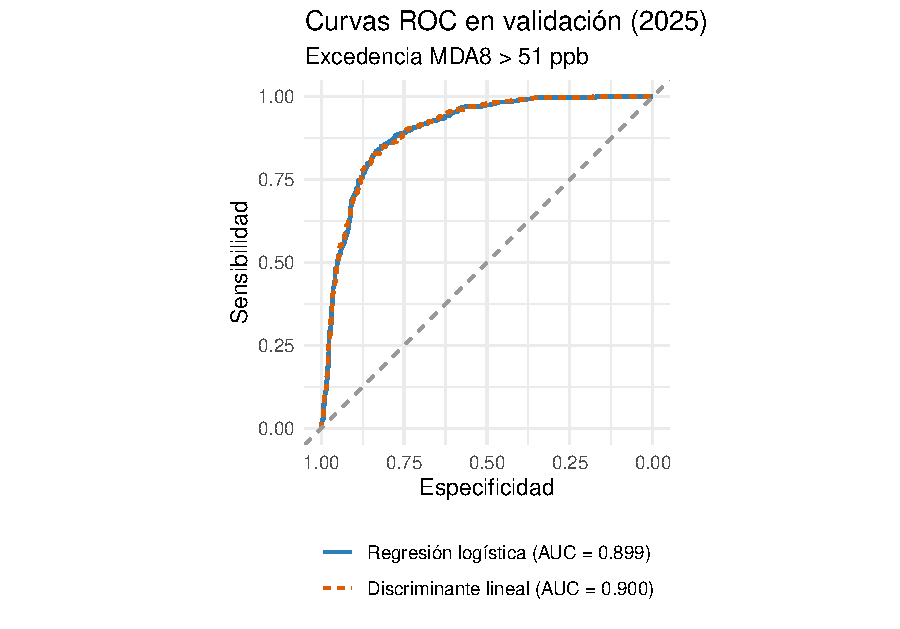
\includegraphics[width=\linewidth]{roc_modelos.pdf}
  \caption{Curvas ROC de ambos modelos en la partición de validación (2025).
    Las dos curvas se superponen; el discriminante se traza punteado.}
  \label{fig:roc-modelos}
\end{figure}

\begin{figure}[t]
  \centering
  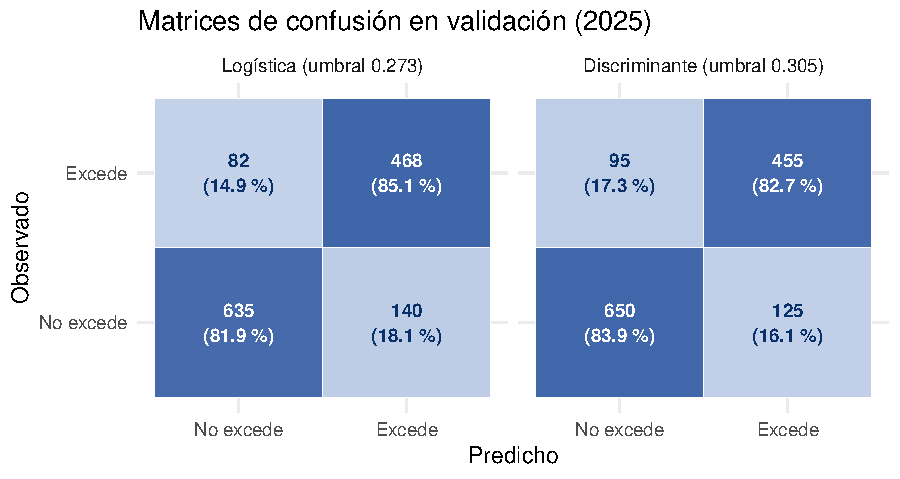
\includegraphics[width=\linewidth]{matriz_confusion.pdf}
  \caption{Matrices de confusión en validación, cada modelo a su propio umbral
    de Youden. Los porcentajes son proporciones por fila (clase observada).}
  \label{fig:matrices}
\end{figure}

Esta coincidencia es el resultado relevante: la heterocedasticidad
documentada en \cref{sec:lda} es real y aun así no altera el desempeño, de
modo que la frontera de decisión que ambos trazan es la misma y la
interpretación de las razones de momios no depende del supuesto de
normalidad que el discriminante exige y la logística no. Como contraste
adicional, la logística sobre las puntuaciones del ACP alcanza 0.848 de AUC
(DeLong $p=0.44$ contra 0.850): los factores no pierden capacidad
discriminante y ganan interpretabilidad.

\paragraph{Corrección de la tasa de error.} El error aparente por
resustitución (0.229 en la logística, 0.230 en el discriminante) apenas se
mueve con validación cruzada de 10 pliegues por días completos (0.231 y
0.232) ni con el método de Lachenbruch (0.231): con 16 parámetros sobre
15,704 observaciones el optimismo es del orden de $p/n$ y ninguno de los dos
clasificadores sobreajusta. Lo que sí revela la validación cruzada es el
efecto de año: dentro de 2021--2024 el AUC fuera de muestra es 0.80, no
0.85. Por año, cada uno predicho por un modelo que no lo vio, 2021--2023
quedan en 0.76--0.77, 2024 sube a 0.84 y 2025 a 0.85. El desempeño esperado
en un año cualquiera es 0.80; el 0.85 corresponde a los dos años de ozono
alto.

\subsubsection{Limitaciones}\label{sec:limitaciones-clasificacion}

\textbf{Autocorrelación.} Las 18,631 filas día-estación de ajuste y
validación no son independientes: la $n$ efectiva está más cerca de los
1,826 días distintos. La correlación entre estaciones dentro de un mismo día
promedia 0.53 en la respuesta y llega a 0.85 en el factor fotoquímico; la
autocorrelación de la respuesta a un día de distancia, dentro de cada
estación, es 0.49. Los errores estándar se corrigieron por conglomerado de
día y las conclusiones sobreviven; lo que no puede corregirse bien es la
dimensión de estación. El AUC no se ve afectado, porque se calcula sobre
observaciones no vistas.

\textbf{Ausencia de compuestos orgánicos volátiles.} Los ejes se describen
como consistentes con combustión primaria, ventilación o forzamiento
fotoquímico, nunca como una atribución de régimen NOx--COV. Una razón de
momios de 2.78 dice que los días con más forzamiento fotoquímico tienen
mayores momios de excedencia; no dice cuál precursor limita la formación de
ozono, pregunta que no es contestable con estos datos.

\textbf{Alcance explicativo.} Los predictores son del mismo día que la
respuesta: los modelos describen qué condiciones acompañan a una excedencia
y no anticipan el ozono del día siguiente.

\textbf{Validación en un año atípico.} 2025 tiene 44\,\% de excedencia
contra 29\,\% del ajuste. El AUC amortigua el sesgo de tasa base, pero la
sensibilidad y la especificidad se leen sobre un año con más días propensos
a excedencia que el promedio de la serie.
   % \subsection
\subsection{Modelo autorregresivo logístico}\label{sec:autorregresivo}

Un modelo autorregresivo explica el valor presente de una serie a partir de
sus propios valores pasados. En su forma clásica, AR($p$), la observación
$y_t$ es una combinación lineal de los $p$ rezagos $y_{t-1},\dots,y_{t-p}$
más ruido. Aquí la respuesta es binaria (día de excedencia o no), así que la
dependencia temporal no puede entrar como media lineal; entra como término
del predictor de una regresión logística:
\begin{equation}
  \operatorname{logit} P(y_t = 1 \mid y_{t-1}, x_t)
    = x_t'\beta + \sum_{i=1}^{p} \alpha_i\, y_{t-i},
  \label{eq:arlog}
\end{equation}
donde $x_t$ reúne los tres puntajes factoriales del mismo día
(\cref{sec:analisis-factorial}) y los armónicos anual y semianual del
calendario. La \cref{sec:serie-tiempo} mostró que la autocorrelación de
rezago 1 sobrevive a la descomposición estacional; \cref{eq:arlog} es la
forma de aprovecharla en lugar de declararla como limitación, como se hizo en
\cref{sec:limitaciones-clasificacion}.

\subsubsection{Proceso}

El modelo se ajusta sobre la serie diaria de área metropolitana construida en
\cref{sec:serie-tiempo}, con $y_t = 1$ cuando al menos la mitad de las
estaciones que reportan excede el umbral de \texttt{excede\_anio\_5}. No se
modela la fracción de estaciones como binomial: la correlación transversal
produce una sobredispersión de 5.97, que subestimaría los errores estándar
por un factor de 2.4. El ajuste usa 2021--2024 y la validación 2025, la misma
partición que \cref{sec:clasificacion_tecs}. La especificación sale de cuatro
diagnósticos, no de una elección a mano:

\begin{enumerate}
  \item \textbf{Orden $p$.} La PACF de $y_t$ corta después del primer rezago
    (0.463 en el rezago 1, 0.100 en el 2) y el BIC, condicionado a las
    covariables, se minimiza en $p=1$. El rezago sobrevive a los factores
    contemporáneos ($LR = 71.4$, 1 g.l.): la persistencia no es un reflejo de
    que la meteorología sea persistente.
  \item \textbf{Estacionariedad.} Una serie binaria no puede tener raíz
    unitaria; lo que se verifica es homogeneidad temporal. El coeficiente
    autorregresivo no cambia entre 2021--2023 y 2024 ($p=0.64$), pero el
    nivel sí: una indicadora de 2024 en adelante es significativa
    ($p=0.0013$). Es un escalón que los factores no absorben y se declara
    como limitación.
  \item \textbf{Forma del predictor.} El \emph{linktest} rechaza sin
    curvatura y deja de rechazar ($p=0.60$) al incluir los cuadrados de
    ventilación y forzamiento fotoquímico, cuyos signos negativos indican
    saturación del efecto. El \emph{link} logit es correcto.
  \item \textbf{Dependencia residual.} Con el rezago, la autocorrelación de
    los residuales de Pearson en el rezago 1 cae de 0.212 a 0.025. Queda un
    residuo de 0.099 en el rezago 2 que no justifica un segundo rezago.
\end{enumerate}

\subsubsection{Resultados e interpretación}

Los coeficientes se leen como razones de momios, igual que en la
\cref{tab:momios-log}, y ningún intervalo del 95\,\% cruza el 1. Haber
excedido el día anterior multiplica los momios de exceder hoy por 3.83: es
el efecto que justifica el término autorregresivo. Entre los factores, el
forzamiento fotoquímico es el de mayor efecto (3.69 por desviación
estándar), seguido de la combustión primaria (2.37); la ventilación es el
único factor protector (0.32). Los cuadráticos quedan por debajo de 1 (0.70
y 0.69): el efecto marginal disminuye cuando el factor ya es alto.

\begin{figure}[t]
  \centering
  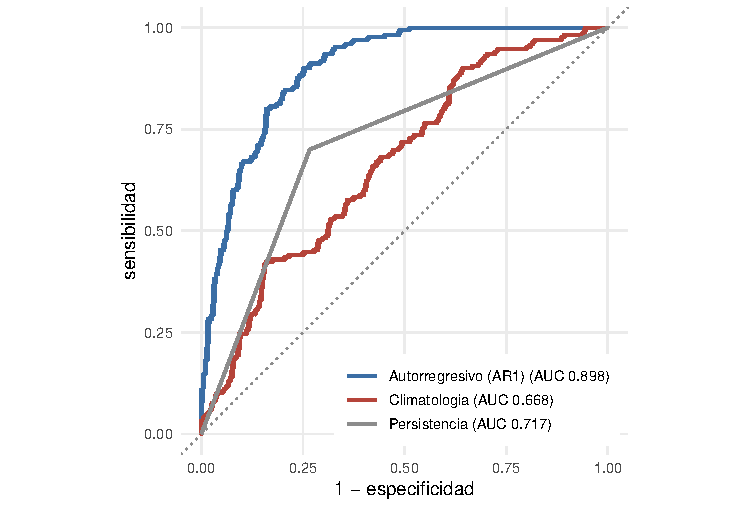
\includegraphics[width=\linewidth]{nowcast_roc.pdf}
  \caption{Curvas ROC en validación (2025) del modelo autorregresivo y de
    las dos líneas base. La persistencia produce tres vértices porque su
    predictor es binario.}
  \label{fig:nowcast-roc}
\end{figure}

Un AUC alto no basta; hay que compararlo contra lo que se obtendría sin
modelo. Las dos líneas base son la climatología (solo el calendario, AUC
0.668) y la persistencia (hoy será como ayer, AUC 0.717). El modelo alcanza
0.898 en 2025 y supera a ambas con $p<10^{-5}$ en la prueba de DeLong
(\cref{fig:nowcast-roc}). Con el umbral de Youden fijado sobre el ajuste
(0.327), no sobre la validación, la sensibilidad es de 0.759 y la
especificidad de 0.841: de 170 días de excedencia detecta 129, con 31 falsas
alarmas en 195 días limpios.

La validación cruzada dejando un año fuera separa el desempeño de la
partición del esperado en un año cualquiera: el AUC va de 0.840 (2021) a
0.915 (2024), con un agrupado de 0.878, IC 95\,\% $[0.859, 0.897]$. Esa
segunda cifra es la estimación de generalización; el 0.898 de 2025 cae
dentro del rango. El efecto de año no se explica por la prevalencia ni por la
cobertura de estaciones y es la limitación principal del modelo.

Dos precisiones acotan la lectura. El modelo subpredice en 2025 (media
predicha 0.338 contra 0.466 observado) por el escalón de nivel de 2024, y no
se recalibra porque sería ajustar un parámetro al periodo de prueba. Y es
\emph{nowcasting}, no pronóstico: los factores son del mismo día que la
respuesta, de modo que el modelo distingue días dentro de una temporada ---lo
que la climatología no puede hacer--- pero no anticipa el ozono de mañana.
 % \subsection

% 6. Resultados
% Seccion 6 de la rubrica. Cada tecnica ya reporta e interpreta sus propios
% resultados en la seccion 5; aqui se consolidan en una sola tabla para que
% sean comparables, sin repetir la interpretacion.

\section{Resultados}
\label{sec:resultados}

La \cref{tab:resultados} consolida el desempeño de los tres clasificadores
sobre la validación de 2025 junto con las dos líneas base del modelo
autorregresivo, y la \cref{tab:resultados-ejes} resume lo que cada técnica
de interdependencia entregó. Los tres clasificadores superan el criterio de
logro de 0.75 fijado en \cref{sec:obj:objetivo}.

\begin{table}[t]
  \centering
  \caption{Desempeño en la validación de 2025. Los modelos día-estación
    (logística y discriminante) y el modelo de área metropolitana
    (autorregresivo y sus líneas base) responden preguntas distintas y sus
    AUC no son directamente comparables entre bloques. Sensibilidad y
    especificidad al umbral de Youden fijado en el ajuste; la
    generalización es el AUC fuera de muestra por validación cruzada
    dejando un año fuera.}
  \label{tab:resultados}
  \small
  \begin{tabular}{lrrrr}
    \toprule
    Modelo & AUC & Sens. & Esp. & General. \\
    \midrule
    \multicolumn{5}{l}{\emph{Día-estación} ($n=2{,}927$)} \\
    Regresión logística    & 0.850 & 0.698 & 0.853 & 0.80 \\
    Discriminante lineal   & 0.846 & 0.758 & 0.788 & 0.80 \\
    \midrule
    \multicolumn{5}{l}{\emph{Área metropolitana} ($n=365$)} \\
    Autorregresivo AR(1)   & 0.898 & 0.759 & 0.841 & 0.878 \\
    Climatología (base)    & 0.668 & ---   & ---   & --- \\
    Persistencia (base)    & 0.717 & ---   & ---   & --- \\
    \bottomrule
  \end{tabular}
\end{table}

\begin{table}[t]
  \centering
  \caption{Ejes retenidos por las técnicas de interdependencia sobre el
    ajuste 2021--2024. Varianza: total en el ACP, común en el AF.}
  \label{tab:resultados-ejes}
  \small
  \begin{tabular}{llr}
    \toprule
    Técnica & Eje & Var. (\%) \\
    \midrule
    \multirow{3}{*}{ACP (15 variables)}
      & Carga primaria de combustión & 26.1 \\
      & Forzamiento fotoquímico      & 19.8 \\
      & Estancamiento atmosférico    & 10.0 \\
    \midrule
    \multirow{3}{*}{AF (13 variables)}
      & Combustión primaria          & 15.7 \\
      & Ventilación                  & 14.5 \\
      & Forzamiento fotoquímico      & 10.1 \\
    \bottomrule
  \end{tabular}
\end{table}

Cuatro resultados atraviesan las técnicas. Primero, los mismos tres ejes
aparecen por dos caminos distintos, y el AF corrige al ACP en un punto: el
eje de estancamiento era un eje de viento, porque la presión barométrica
tiene comunalidad de 0.13 y casi toda su varianza es específica. Segundo, la
jerarquía de efectos es estable en los tres clasificadores: el forzamiento
fotoquímico pesa más que la combustión primaria, la ventilación protege, y
en los modelos día-estación la temporada y la zona pesan más que cualquier
factor. Tercero, la dependencia temporal es real y aprovechable: el rezago
de la respuesta sube el AUC de área metropolitana de 0.882 a 0.898 y
multiplica los momios por 3.83. Cuarto, todos los modelos comparten un
efecto de año que ningún predictor explica: 2024 y 2025 son los años de
ozono más alto de la serie y también los mejor clasificados, y el desempeño
esperado en un año cualquiera queda entre 0.04 y 0.05 por debajo del de la
validación.


% 7. Discusión y conclusiones
% Seccion 7 de la rubrica: discusion y conclusiones (1 a 2 paginas), con los
% resultados mas relevantes, recomendaciones y las preguntas nuevas que deja
% el analisis.

\section{Discusión y conclusiones}
\label{sec:conclusiones}

\subsection{Discusión}

El objetivo era clasificar cada día-estación como excedencia o no del MDA8
a 51 ppb a partir de las condiciones del mismo día, con AUC de al menos
0.75, e identificar las condiciones latentes que explican esa
clasificación. Se cumple: los tres clasificadores superan el criterio, y las
técnicas de interdependencia producen tres ejes con lectura física estable
fuera del periodo de ajuste.

La excedencia de ozono en el AMM es, ante todo, un fenómeno estacional y
regional. La temporada es el predictor de mayor efecto en los modelos
día-estación ---la primavera triplica los momios del invierno--- y el
forzamiento fotoquímico, el eje de temperatura, radiación y sequedad, es el
factor continuo dominante. Que el forzamiento pese más que la carga de
precursores es coherente con la química del ozono como contaminante
secundario: los ingredientes son necesarios, pero es la energía disponible
la que fija la velocidad de las reacciones. La ventilación es el único
mecanismo protector medido, y el AF muestra que es el viento, no la presión,
lo que define ese eje.

Sobre ese fondo estacional hay una señal espacial que la meteorología medida
no explica. A igual temporada y condiciones, el Noroeste y el Suroeste casi
cuadruplican los momios del Noreste, y la tasa de excedencia de una estación
correlaciona 0.83 con su elevación. El viento predominante del oriente
arrastra los precursores hacia el pie de la sierra, donde la orografía frena
su salida; el ordenamiento poniente--oriente es estable en las cuatro
temporadas. Los contrastes de zona descansan, sin embargo, en 15 unidades
espaciales, y su precisión es la que 15 unidades pueden dar.

La dependencia temporal es el tercer hallazgo. La autocorrelación de un día
para otro sobrevive a la descomposición estacional en las cuatro series de
área metropolitana, y un solo rezago de la respuesta captura casi toda esa
dependencia: haber excedido ayer casi cuadruplica los momios de exceder hoy,
controlando por factores y calendario. El modelo autorregresivo distingue
días dentro de una temporada, lo que la climatología no puede hacer.

Dos limitaciones acotan todo lo anterior. La primera es el efecto de año:
2024 y 2025 tienen un nivel de excedencia que los factores no explican, y
ningún modelo generaliza igual de bien a 2021 que a 2024. Con estos datos
no puede decidirse si es un cambio de emisiones, de instrumentación o dos
años meteorológicamente atípicos. La segunda es la ausencia de compuestos
orgánicos volátiles: sin ellos, los ejes se describen como consistentes con
combustión, ventilación o fotoquímica, y ninguna afirmación sobre el régimen
que limita la formación de ozono es contestable.

\subsection{Conclusiones}

\begin{enumerate}[label=\roman*.]
  \item Los tres clasificadores alcanzan AUC de 0.846 a 0.898 en 2025 y
    superan el criterio de logro. La logística y el discriminante son
    equivalentes en la práctica, de modo que la interpretación de las razones
    de momios no depende del supuesto de normalidad.
  \item La excedencia es principalmente estacional: la temporada pesa más
    que cualquier factor continuo, y entre estos domina el forzamiento
    fotoquímico (2.78 por desviación estándar) sobre la combustión primaria
    (1.92); la ventilación protege (0.90).
  \item Existe una señal espacial no explicada por la meteorología medida:
    el poniente del AMM casi cuadruplica los momios del Noreste, en
    correspondencia con la elevación y el viento predominante.
  \item El calendario laboral apenas influye; solo el domingo tiene un
    efecto claro y pequeño, y el del sábado desaparece al corregir los
    errores estándar por dependencia.
  \item La dependencia día a día es genuina y un modelo AR(1) la aprovecha:
    supera a la climatología y a la persistencia con generalización esperada
    de 0.878.
\end{enumerate}

\subsection{Recomendaciones}

Para la gestión de la calidad del aire, el modelo autorregresivo sobre la
serie de área metropolitana puede operar como sistema de \emph{nowcasting}
de excedencia con las mediciones del propio día, con un umbral de decisión
que privilegie la sensibilidad, porque el costo de no avisar de un día malo
supera al de una alerta de más. Las zonas Noroeste y Suroeste merecen
vigilancia y medidas de control específicas, ya que su riesgo excede lo que
explican sus condiciones meteorológicas. Y la incorporación de mediciones de
compuestos orgánicos volátiles a la red del SIMA es la única vía para pasar
de asociaciones a mecanismo.

Para el análisis, tres mejoras metodológicas quedan identificadas: estimar
el parámetro de Box-Cox solo sobre el ajuste, para cerrar la única fuga que
persiste; incluir un término de media móvil sobre los residuales, que el
residuo de segundo orden del modelo autorregresivo justifica; y extender el
modelo a pronóstico rezagando los factores, con validación propia.

\subsection{Preguntas nuevas}

\begin{itemize}
  \item ¿Qué produjo el escalón de 2024? Distinguir entre cambio de
    emisiones, de instrumentación y años atípicos exige inventarios de
    emisiones y bitácoras de calibración que este trabajo no tuvo.
  \item ¿Qué característica del poniente explica el exceso de riesgo que
    la zona conserva tras controlar por meteorología? Uso de suelo,
    distancia a fuentes industriales y recirculación orográfica son las
    candidatas.
  \item ¿Cuánto del efecto de la temporada es fotoquímica y cuánto es
    régimen de vientos? Los factores lo capturan en parte, pero la temporada
    conserva un efecto propio que sugiere una variable estacional no medida.
  \item ¿Hasta qué horizonte es útil el pronóstico? El tiempo de mezcla de
    1.3 días de la cadena binaria sugiere que más allá de dos o tres días la
    predicción converge a la climatología del mes.
\end{itemize}


\section{Declaratoria de uso de inteligencia artificial}
\label{sec:declaratoria-ia}

Se utilizó inteligencia artificial generativa de la siguiente forma
(opción B):

\begin{description}[leftmargin=0pt, labelindent=0pt, style=nextline]
  \item[Herramienta] Claude (Anthropic), a través de la interfaz Claude Code.
  \item[Uso realizado] Asistencia en la escritura y depuración del código de
    consolidación, limpieza y análisis en Python y R; redacción y revisión
    de estilo de las secciones de este reporte; y revisión automática de
    las solicitudes de incorporación del repositorio. El registro de esas
    intervenciones queda en el historial de \emph{commits} y en los hilos de
    revisión, ambos públicos en el repositorio citado al final del
    documento.
  \item[Secciones donde se utilizó] Todas las secciones del reporte
    recibieron revisión de estilo; el código de \cref{sec:preparacion-datos}
    a \cref{sec:modelacion} recibió asistencia de depuración.
  \item[Validación realizada por los estudiantes] El planteamiento del
    objetivo, la selección de las técnicas, los criterios de decisión y la
    interpretación de los resultados son autoría del equipo. Ninguna cifra
    del documento proviene del modelo: todas se obtuvieron de la ejecución
    de las notebooks y se verificaron contra sus salidas. El equipo revisó,
    verificó y asume la responsabilidad del contenido final entregado.
\end{description}


\printbibliography

% --- Anexos ---
% Solo informacion complementaria citada desde el cuerpo: las tecnicas que se
% probaron y descartaron (\cref{sec:tecnicas-descartadas}) y los diccionarios
% de datos (\cref{sec:diccionario,sec:diccionario-transformado}). No cuentan
% contra el limite de paginas del cuerpo.
\appendix
\section{Técnicas y decisiones descartadas}\label{sec:tecnicas-descartadas}

El análisis factorial (\cref{sec:af}) generó, además de su resultado final,
tres decisiones metodológicas que se probaron y se rechazaron de forma
explícita, y dos variables que el modelo no toleró. Documentarlas evita que
parezcan omisiones: cada una se descartó por una razón concreta y verificable,
no por conveniencia.

\subsection{Análisis paralelo de Horn}

Es el criterio estándar para decidir cuántos factores retener, y aquí retiene
siete --- el doble que el MAP de Velicer finalmente adoptado
(\cref{fig:af-paralelo}). No se sigue, porque el resultado es un artefacto del
tamaño muestral y no una señal sustantiva: el umbral simulado sobre la matriz
reducida se sitúa en 0.06 y sobre la completa en 1.06. Con las 16,008
observaciones de entrenamiento del bloque de 14 predictores, los eigenvalores que produciría ruido puro se concentran
fortísimo alrededor de su valor esperado, la banda de simulación se angosta
casi a un punto, y cualquier eigenvalor apenas positivo la supera. El
argumento para descartarlo se sostiene mirando los umbrales simulados, sin
necesidad de ver una sola carga factorial. El MAP de Velicer se usa en su
lugar por ser un mínimo descriptivo que no lleva $n$ en la fórmula y no se
infla con el tamaño de la muestra.

\subsection{Extracción por máxima verosimilitud}

La extracción de \cref{sec:af} usa ejes principales iterados y no máxima
verosimilitud, que exige normalidad multivariada. Las transformaciones
Box-Cox de \cref{sec:transformaciones} acercaron las marginales a la simetría
($|\text{sesgo}|<0.5$) pero no las volvieron normales, de modo que ese
supuesto no se sostiene sobre estos datos. La solución de ejes principales se
validó contra \texttt{psych::fa(fm="pa", rotate="varimax")} de R sobre el
mismo bloque: coincide hasta orden y signo de los factores, con comunalidades
iguales a la milésima.

\subsection{Rotación oblicua}

Antes de adoptar varimax se probó una rotación oblicua (oblimin), que permite
correlación entre factores. Encontró correlaciones de hasta 0.32 entre ellos
--- físicamente razonable, ya que el viento dispersa contaminantes y no es
independiente de la carga de combustión. Se rechaza para el uso instrumental
de los puntajes: el objetivo de \cref{sec:clasificacion_tecs} es disponer de
predictores no colineales, y una solución oblicua reintroduce exactamente el
problema de multicolinealidad que el análisis factorial vino a resolver. La
correlación entre factores se reporta como hallazgo, pero no se lleva al
modelo de clasificación.

\subsection{Dos variables que el modelo factorial no toleró}

\texttt{NOX} y \texttt{RH\_min\_diurna} produjeron comunalidades mayores que 1
--- los llamados \textbf{casos Heywood}, imposibles porque la comunalidad es
una proporción de varianza. \texttt{NOX} es, por definición química, la suma
de \texttt{NO} y \texttt{NO2} ($r=0.985$ contra esa suma): no es una variable
redundante en un sentido estadístico ordinario, es una identidad contable que
el PCA de \cref{sec:pca} absorbió sin protestar y que el análisis factorial no
puede repartir en comunalidad y unicidad. \texttt{RH\_min\_diurna}
correlaciona 0.892 con \texttt{RH\_media}; a diferencia de \texttt{NOX} no es
una identidad, así que \cref{sec:af} la dejó en observación hasta que el
segundo ajuste, ya con el diagnóstico completo, forzó la misma salida. Ambas
se eliminaron del bloque de predictores, que queda en 13 variables con un VIF
máximo de 2.54. Que el PCA no haya señalado ninguno de los dos problemas es en
sí mismo un resultado: el modelo factorial expone redundancias que la
descomposición de varianza total no tiene forma de reportar.

% =============================================================================
%  Seccion: Diccionario de datos
%
%  Version en LaTeX de docs/Diccionario_Sima.md. Si cambia el consolidado,
%  hay que actualizar AMBOS archivos (el .md es el que se consulta al programar).
%
%  Este archivo NO lleva preambulo: main.tex lo mete con \input. Solo usa
%  paquetes que main.tex ya carga (booktabs, amsmath, cleveref). Si hace falta
%  uno nuevo, se pide en una issue de main.tex; no se agrega aqui.
%
%  Las tablas anchas usan el entorno table* (flotante a dos columnas): en un
%  documento 5p una tabla de 6 o 7 columnas no cabe en una sola columna. Los
%  flotantes a dos columnas SOLO pueden ir arriba de la pagina, por eso llevan
%  [t] y no [h].
% =============================================================================

\section{Diccionario de datos}\label{sec:diccionario}

Esta seccion documenta el consolidado que produce
\texttt{src/importar\_datos.py} a partir de los seis libros anuales del SIMA
(\texttt{data/raw/BD 2020.xlsx} a \texttt{data/raw/BD 2025.xlsx}): que contiene
cada variable, como estan cubiertas las estaciones y que anomalias de calidad
hay que atender antes de cualquier analisis multivariado.

\subsection{Dimension del conjunto de datos}\label{sec:dic:dimension}

El consolidado tiene 754\,603 filas y 18 columnas: 3 identificadoras y 15
parametros medidos. Cada fila es una estacion en una hora, la cobertura va del
1 de enero de 2020 a las 00:00 al 31 de diciembre de 2025 a las 23:00, y no hay
registros duplicados. De las 11\,319\,045 celdas de parametros, 1\,188\,343
estan vacias: un 10.50\,\% de faltantes.

En el origen cada libro anual trae una hoja por estacion --- 13 en 2020, 14 en
2021 y 15 de 2022 en adelante --- en formato ancho: una fila por hora y una
columna por parametro. No existe una columna de estacion; la consolidacion
promueve el nombre de la hoja a la columna \texttt{estacion} y apila los seis
anios.

\subsection{Variables identificadoras}\label{sec:dic:identificadoras}

\begin{description}
  \item[\texttt{fecha}] Marca temporal de la observacion, con resolucion
    horaria (\texttt{datetime64}), de 2020-01-01 00:00 a 2025-12-31 23:00. Sin
    faltantes.
  \item[\texttt{estacion}] Categorica nominal de 15 niveles: CE, NE, NE2, NE3,
    NO, NO2, NO3, NTE, NTE2, SE, SE2, SE3, SO, SO2 y SUR. Sin faltantes.
  \item[\texttt{anio}] Anio calendario, derivado del archivo de origen.
    Numerica discreta (o categorica ordinal), con valores de 2020 a 2025. Sin
    faltantes.
\end{description}

\subsection{Contaminantes criterio}\label{sec:dic:contaminantes}

Los ocho contaminantes criterio son numericos continuos y se resumen en
\cref{tab:dic-contaminantes}. El rango de operacion que se reporta abarca desde
el anio mas restrictivo hasta el mas permisivo del periodo, porque el limite
cambia anio con anio (\cref{sec:dic:centinela}). Segun \texttt{Etiquetas.xlsx},
O$_3$, SO$_2$ y NO$_2$ pueden pasarse a ppm dividiendo entre 1000.

\subsection{Parametros meteorologicos}\label{sec:dic:meteorologicos}

Los siete parametros meteorologicos aparecen en \cref{tab:dic-meteo}. Dos de
ellos no pueden tratarse como variables continuas ordinarias:

\begin{itemize}
  \item \texttt{WDR} es una variable \textbf{circular}, aunque se almacene como
    numero: $0^{\circ}$ y $360^{\circ}$ son la misma direccion (norte). No
    puede promediarse, escalarse ni correlacionarse como las demas; hay que
    descomponerla en $\sin\theta$ y $\cos\theta$, o bien en las componentes de
    viento $u = -\,\mathrm{WSR}\cdot\sin\theta$ y
    $v = -\,\mathrm{WSR}\cdot\cos\theta$. Es un atributo derivado que debe
    construirse en la etapa de transformacion.
  \item \texttt{RAINF} y \texttt{SR} son de \textbf{cero inflado}: el 98.4\,\%
    de los registros validos de precipitacion y el 39.6\,\% de los de radiacion
    solar valen exactamente cero (noche y dias sin lluvia). Son ceros
    legitimos, no faltantes ni errores, pero rompen los supuestos de normalidad
    y distorsionan cualquier estandarizacion.
\end{itemize}

\subsection{Catalogo de estaciones}\label{sec:dic:estaciones}

\Cref{tab:dic-estaciones} lista las 15 estaciones y su cobertura calculada
sobre el consolidado. Dos estaciones no estan documentadas en el catalogo del
SIMA y ademas entraron tarde a la red: NE3 aparece a partir de 2021 y NO3
hasta diciembre de 2022, de modo que cualquier analisis que exija el panel
completo debe excluirlas o recortarse al periodo comun.

\subsection{Faltantes}\label{sec:dic:faltantes}

\Cref{tab:dic-faltantes} da el porcentaje de nulos por variable, que va del
3.66\,\% de \texttt{SR} al 25.23\,\% de \texttt{PM2.5}. Ese promedio esconde lo
importante: el faltante no esta repartido de forma pareja entre estaciones ni
entre anios. Para el ozono, 2020 es practicamente inservible: varias
estaciones (NTE, SUR, SE2, NE, NO) superan el 98\,\% de faltante ese anio; de
2022 en adelante el faltante de O$_3$ baja a entre 1\,\% y 8\,\% en casi toda
la red.

Los faltantes de este conjunto \textbf{no son aleatorios} (no son MCAR): el
SIMA invalida horas por calibracion, falla o condicion anomala antes de
entregar los archivos, y esas horas quedan como celda vacia sin que el motivo
sea recuperable. Esto acerca el mecanismo a MAR, lo que condiciona que
imputacion resulta defendible y debe declararse como supuesto.

\subsection{Valores centinela y fisicamente imposibles}\label{sec:dic:centinela}

Ademas de los faltantes explicitos, el consolidado contiene valores que no
pueden tomarse como mediciones: el codigo $-9999$ del \emph{datalogger} (26
celdas entre NOX, RAINF, RH, SR, TOUT, WSR y WDR), porcentajes de humedad
relativa mayores a 100\,\%, y lecturas fuera del rango fisico del sensor (por
ejemplo, TOUT $>50^{\circ}$C o WSR $>100$ km/h). Estos valores se convierten a
\texttt{NaN} antes de cualquier calculo, usando como filtro duro el
\textbf{rango de fabricante} de cada sensor (\cref{tab:dic-fabricante}), que es
fisico y estable. El rango de operacion anual que declara el SIMA no se usa
para este filtro porque es inconsistente entre anios (en 2022, por ejemplo,
declara para \texttt{PRS} un minimo mas alto que en 2021 y 2023, lo que
borraria datos validos); se trata en cambio como senial de sospecha a
revisar, no como regla de borrado automatico.

% -----------------------------------------------------------------------------
%  Tablas
% -----------------------------------------------------------------------------

\begin{table*}[t]
  \centering
  \caption{Contaminantes criterio. Todas son variables numericas continuas. El
    rango de operacion va del anio mas restrictivo al mas permisivo del
    periodo.}
  \label{tab:dic-contaminantes}
  \small
  \begin{tabular}{lllcccc}
    \toprule
    Variable & Descripcion & Unidad & Rango de operacion & Rango observado & Mediana & \% nulos \\
    \midrule
    \texttt{CO}    & Monoxido de carbono                   & ppm             & 0--8 a 0--20       & $0.0$--$37.0$    & 1.17  & 13.31 \\
    \texttt{NO}    & Monoxido de nitrogeno                 & ppb             & 0--350 a 0--500    & $0.3$--$945.1$   & 5.00  & 16.75 \\
    \texttt{NO2}   & Dioxido de nitrogeno                  & ppb             & 0--100 a 0--200    & $0.0$--$188.6$   & 11.40 & 17.37 \\
    \texttt{NOX}   & Oxidos de nitrogeno (NO $+$ NO$_2$)   & ppb             & 0--400 a 0--500    & $-9999$--$971.8$ & 17.30 & 16.82 \\
    \texttt{O3}    & \textbf{Ozono}: variable objetivo     & ppb             & 0--153 a 0--185    & $0.5$--$265.0$   & 23.00 & 14.73 \\
    \texttt{PM10}  & Particulas $<10\,\mu$m                & $\mu$g/m$^3$    & 0--800 a 0--999    & $1.0$--$1001.0$  & 49.00 & 4.63  \\
    \texttt{PM2.5} & Particulas $<2.5\,\mu$m               & $\mu$g/m$^3$    & 0--205.94 a 0--999 & $0.0$--$999.0$   & 17.00 & 25.23 \\
    \texttt{SO2}   & Dioxido de azufre                     & ppb             & 0--150 a 0--405    & $0.0$--$404.7$   & 3.80  & 15.03 \\
    \bottomrule
  \end{tabular}
\end{table*}

\begin{table*}[t]
  \centering
  \caption{Parametros meteorologicos. Todas son variables numericas continuas,
    con las salvedades de \texttt{WDR} (circular) y de \texttt{RAINF} y
    \texttt{SR} (cero inflado).}
  \label{tab:dic-meteo}
  \small
  \begin{tabular}{lllcccc}
    \toprule
    Variable & Descripcion & Unidad & Rango de operacion & Rango observado & Mediana & \% nulos \\
    \midrule
    \texttt{TOUT}  & Temperatura ambiente & $^{\circ}$C        & $-6.5$--45 a 0--45.5 & $-9999$--$785.0$ & 24.02  & 6.95  \\
    \texttt{RH}    & Humedad relativa     & \%                 & 0--100               & $-9999$--$725.0$ & 59.00  & 11.38 \\
    \texttt{SR}    & Radiacion solar      & kW/m$^2$           & 0--1 a 0--1.26       & $-9999$--$604.0$ & 0.00   & 3.66  \\
    \texttt{RAINF} & Precipitacion        & mm/h               & 0--25 a 0--80        & $-9999$--$360.0$ & 0.00   & 4.74  \\
    \texttt{PRS}   & Presion atmosferica  & mmHg               & 687.5--750           & $0.0$--$750.0$   & 714.40 & 5.08  \\
    \texttt{WSR}   & Velocidad del viento & km/h               & 0--35 a 0--75        & $-9999$--$337.0$ & 7.40   & 6.87  \\
    \texttt{WDR}   & Direccion del viento & grados azimutales  & 0--360               & $-9999$--$360.0$ & 116.00 & 8.35  \\
    \bottomrule
  \end{tabular}
\end{table*}

\begin{table}[t]
  \centering
  \caption{Catalogo de estaciones de monitoreo y su cobertura, calculada
    sobre el consolidado.}
  \label{tab:dic-estaciones}
  \small
  \begin{tabular}{llr}
    \toprule
    Clave & Cobertura & Horas \\
    \midrule
    \texttt{CE}   & 2020--2025                & 52\,605 \\
    \texttt{NE}   & 2020--2025                & 52\,595 \\
    \texttt{NE2}  & 2020--2025                & 52\,593 \\
    \texttt{NE3}  & \textbf{2021--2025}       & 43\,817 \\
    \texttt{NO}   & 2020--2025                & 52\,597 \\
    \texttt{NO2}  & 2020--2025                & 52\,594 \\
    \texttt{NO3}  & \textbf{dic.\ 2022--2025} & 27\,045 \\
    \texttt{NTE}  & 2020--2025                & 52\,595 \\
    \texttt{NTE2} & 2020--2025                & 52\,593 \\
    \texttt{SE}   & 2020--2025                & 52\,599 \\
    \texttt{SE2}  & 2020--2025                & 52\,595 \\
    \texttt{SE3}  & 2020--2025                & 52\,593 \\
    \texttt{SO}   & 2020--2025                & 52\,597 \\
    \texttt{SO2}  & 2020--2025                & 52\,593 \\
    \texttt{SUR}  & 2020--2025                & 52\,592 \\
    \bottomrule
  \end{tabular}
\end{table}

\begin{table}[t]
  \centering
  \caption{Porcentaje de valores faltantes por variable.}
  \label{tab:dic-faltantes}
  \small
  \begin{tabular}{lr@{\qquad}lr}
    \toprule
    Variable & \% nulo & Variable & \% nulo \\
    \midrule
    \texttt{PM2.5} & 25.23 & \texttt{RH}    & 11.38 \\
    \texttt{NO2}   & 17.37 & \texttt{WDR}   & 8.35  \\
    \texttt{NOX}   & 16.82 & \texttt{TOUT}  & 6.95  \\
    \texttt{NO}    & 16.75 & \texttt{WSR}   & 6.87  \\
    \texttt{SO2}   & 15.03 & \texttt{PRS}   & 5.08  \\
    \texttt{O3}    & 14.73 & \texttt{RAINF} & 4.74  \\
    \texttt{CO}    & 13.31 & \texttt{PM10}  & 4.63  \\
                   &       & \texttt{SR}    & 3.66  \\
    \bottomrule
  \end{tabular}
\end{table}

\begin{table}[t]
  \centering
  \caption{Rango de fabricante por parametro, adoptado como filtro duro de
    valores imposibles.}
  \label{tab:dic-fabricante}
  \small
  \begin{tabular}{lc}
    \toprule
    Parametro & Rango de fabricante \\
    \midrule
    PM10, PM2.5, O3      & $0$--$1000$     \\
    NO, NO2, NOx, SO2    & $0$--$500$      \\
    CO                   & $0$--$50$       \\
    RH                   & $0$--$100$      \\
    WS (\texttt{WSR})    & $0$--$180$      \\
    TEMP (\texttt{TOUT}) & $-50$--$50$     \\
    SR                   & $0$--$1.4$      \\
    BP (\texttt{PRS})    & $449.9$--$824.9$\\
    WD (\texttt{WDR})    & $0$--$360$      \\
    \bottomrule
  \end{tabular}
\end{table}


Este es un test
\section{Diccionario de datos transformados}\label{sec:diccionario-transformado}
Esta sección documenta el conjunto de datos diario resultante de las
transformaciones de \cref{sec:transformaciones}. El archivo
\texttt{data/processed/sima\_transformado\_diario.parquet} constituye la entrada
de los análisis multivariados posteriores.

\subsection{Dimensión y cobertura}
El conjunto transformado contiene 26,691 observaciones día-estación y 34
columnas. Comprende 15 estaciones y cubre del 1 de enero de 2021 al 31 de diciembre
de 2025. Se transformaron y estandarizaron 16 predictores continuos medidos. Las
18 columnas restantes se conservaron en su escala original.

El criterio de \cref{sec:transformaciones} se reaplicó sobre la tabla diaria sin
modificar el método. De las 16 variables continuas, 13 requirieron Box-Cox y
estandarización z. \texttt{PRS\_media}, \texttt{RH\_media} y
\texttt{RH\_min\_diurna} cumplieron el criterio de sesgo desde la escala
original y solo se estandarizaron. Los valores faltantes se conservaron sin
imputación.

\subsection{Variables del conjunto diario}
La \cref{tab:dic-diario-continuas} presenta los 16 predictores continuos. Las
unidades corresponden a la escala original, antes de la transformación y la
estandarización.

\begin{table*}[t]
  \centering
  \caption{Predictores continuos transformados y estandarizados del conjunto
    diario. Las unidades corresponden a la escala original.}
  \label{tab:dic-diario-continuas}
  \footnotesize
  \setlength{\tabcolsep}{4pt}
  \begin{tabular}{lp{7.2cm}llr}
    \toprule
    Variable & Descripción & Unidad & Tratamiento & Faltantes \\
    \midrule
    \texttt{TOUT\_max} & Máximo diario de temperatura ambiente
      & $^{\circ}\mathrm{C}$ & Box-Cox + z & 1,561 \\
    \texttt{SR\_acum} & Acumulado diario de radiación solar
      & $\mathrm{kWh}/\mathrm{m}^{2}$ & Box-Cox + z & 1,123 \\
    \texttt{NO\_06\_09} & Media de NO entre las 06:00 y las 09:00 h
      & ppb & Box-Cox + z & 1,757 \\
    \texttt{NO2\_06\_09} & Media de NO$_2$ entre las 06:00 y las 09:00 h
      & ppb & Box-Cox + z & 1,776 \\
    \texttt{NOX\_06\_09} & Media de NO$_x$ entre las 06:00 y las 09:00 h
      & ppb & Box-Cox + z & 1,790 \\
    \texttt{CO\_06\_09} & Media de CO entre las 06:00 y las 09:00 h
      & ppm & Box-Cox + z & 1,937 \\
    \texttt{WSR\_media} & Media diaria de la velocidad del viento
      & km/h & Box-Cox + z & 1,008 \\
    \texttt{WSR\_min} & Mínimo diario de la velocidad del viento
      & km/h & Box-Cox + z & 1,008 \\
    \texttt{PRS\_media} & Media diaria de la presión atmosférica
      & mmHg & solo z & 886 \\
    \texttt{RH\_media} & Media diaria de la humedad relativa
      & \% & solo z & 2,649 \\
    \texttt{RH\_min\_diurna} & Mínimo diurno de la humedad relativa
      & \% & solo z & 2,575 \\
    \texttt{viento\_u\_media} & Media vectorial diaria del viento en la
      componente este-oeste & --- & Box-Cox + z & 1,447 \\
    \texttt{viento\_v\_media} & Media vectorial diaria del viento en la
      componente norte-sur & --- & Box-Cox + z & 1,447 \\
    \texttt{PM10\_media} & Media diaria de partículas PM$_{10}$
      & $\mu\mathrm{g}/\mathrm{m}^{3}$ & Box-Cox + z & 940 \\
    \texttt{PM2.5\_media} & Media diaria de partículas PM$_{2.5}$
      & $\mu\mathrm{g}/\mathrm{m}^{3}$ & Box-Cox + z & 5,965 \\
    \texttt{SO2\_media} & Media diaria de SO$_2$
      & ppb & Box-Cox + z & 1,933 \\
    \bottomrule
  \end{tabular}
\end{table*}

Con el 2025 completo el sesgo de \texttt{SR\_acum} sube a 0.53 y ya no
cumple el criterio, por lo que se transforma ($\lambda=0.755$); se conserva
como predictor continuo y no se convierte en binaria. Las 16 variables de la
\cref{tab:dic-diario-continuas} quedan dentro del criterio
$|\mathrm{sesgo}|<0.5$.

La \cref{tab:dic-diario-originales} reúne las 18 columnas que no se
transformaron. \texttt{msnm} se conserva porque representa un atributo de la
estación, con 15 valores repetidos, y no una medición diaria. \texttt{MDA8} y
\texttt{O3\_max\_1h} permanecen en ppb porque definen las variables objetivo y
sus umbrales deben conservar una interpretación física directa.

\begin{table*}[t]
  \centering
  \caption{Columnas conservadas en la escala original dentro del conjunto
    diario transformado.}
  \label{tab:dic-diario-originales}
  \footnotesize
  \setlength{\tabcolsep}{4pt}
  \begin{tabular}{llp{8.0cm}lr}
    \toprule
    Variable & Tipo & Descripción & Unidad & Faltantes \\
    \midrule
    \texttt{estacion} & nominal & Estación de monitoreo SIMA, con 15 niveles
      & --- & 0 \\
    \texttt{fecha} & fecha & Día calendario de la observación
      & --- & 0 \\
    \texttt{zona} & nominal & Zona geográfica del catálogo SIMA, con siete
      niveles & --- & 0 \\
    \texttt{msnm} & continua & Elevación de la estación sobre el nivel del mar
      & m & 0 \\
    \texttt{anio} & discreta & Año calendario
      & --- & 0 \\
    \texttt{mes} & discreta & Mes calendario
      & --- & 0 \\
    \texttt{temporada} & nominal & Temporada del año, con cuatro niveles
      & --- & 0 \\
    \texttt{tipo\_dia} & nominal & Día laborable, sábado, domingo o festivo
      & --- & 0 \\
    \texttt{festivo} & binaria & Indicadora de día de asueto
      & 0/1 & 0 \\
    \texttt{fin\_de\_semana} & binaria & Indicadora de sábado o domingo
      & 0/1 & 0 \\
    \texttt{llovio} & binaria & Indicadora de al menos una hora del día con
      precipitación & 0/1 & 800 \\
    \texttt{MDA8} & continua & Máximo diario de la media móvil de 8 h de O$_3$
      & ppb & 1,591 \\
    \texttt{ventanas\_validas} & discreta & Número de ventanas móviles de 8 h válidas
      durante el día, de un máximo de 24 & ventanas & 0 \\
    \texttt{O3\_max\_1h} & continua & Máximo horario de O$_3$ durante el día
      & ppb & 838 \\
    \texttt{excede\_anio\_1} & binaria & Excedencia de MDA8 sobre 65 ppb
      & 0/1 & 1,591 \\
    \texttt{excede\_anio\_3} & binaria & Excedencia de MDA8 sobre 60 ppb
      & 0/1 & 1,591 \\
    \texttt{excede\_anio\_5} & binaria & Excedencia de MDA8 sobre 51 ppb
      & 0/1 & 1,591 \\
    \texttt{excede\_1h} & binaria & Excedencia del máximo horario sobre 95 ppb
      & 0/1 & 0 \\
    \bottomrule
  \end{tabular}
\end{table*}

\subsection{Sesgo y curtosis}
La \cref{tab:dic-diario-sesgo} compara la forma de las distribuciones antes y
después del tratamiento. La estandarización z es una transformación lineal y no
modifica el sesgo ni la curtosis. Por ello, las tres variables que solo se
estandarizaron conservan los valores de la escala original.

\begin{table*}[t]
  \centering
  \caption{Sesgo y curtosis de exceso, con referencia normal igual a cero, de
    las variables continuas del conjunto diario antes y después del
    tratamiento.}
  \label{tab:dic-diario-sesgo}
  \small
  \setlength{\tabcolsep}{6pt}
  \begin{tabular}{lrrrrrr}
    \toprule
    & & & \multicolumn{2}{c}{Sesgo} & \multicolumn{2}{c}{Curtosis} \\
    \cmidrule(lr){4-5}\cmidrule(lr){6-7}
    Variable & Despl. & $\lambda$ & Antes & Después & Antes & Después \\
    \midrule
    \texttt{TOUT\_max} & 1.55 & 2.118 & $-0.86$ & $-0.16$ & 0.60 & $-0.49$ \\
    \texttt{SR\_acum} & 1.00 & 0.755 & 0.53 & 0.00 & 3.04 & 0.99 \\
    \texttt{NO\_06\_09} & 0.00 & $-0.103$ & 4.13 & 0.01 & 32.49 & $-0.09$ \\
    \texttt{NO2\_06\_09} & 1.00 & 0.279 & 1.67 & 0.02 & 6.89 & 0.40 \\
    \texttt{NOX\_06\_09} & 0.00 & 0.008 & 3.04 & 0.00 & 17.68 & 0.52 \\
    \texttt{CO\_06\_09} & 1.00 & $-0.320$ & 1.42 & 0.02 & 4.82 & $-0.53$ \\
    \texttt{WSR\_media} & 0.00 & 0.134 & 8.29 & 0.07 & 149.74 & 3.94 \\
    \texttt{WSR\_min} & 0.00 & 0.285 & 8.74 & 0.04 & 347.89 & 0.94 \\
    \texttt{PRS\_media} & --- & --- & 0.12 & 0.12 & $-0.16$ & $-0.16$ \\
    \texttt{RH\_media} & --- & --- & $-0.37$ & $-0.37$ & 0.19 & 0.19 \\
    \texttt{RH\_min\_diurna} & --- & --- & 0.45 & 0.45 & 0.15 & 0.15 \\
    \texttt{viento\_u\_media} & 116.16 & 2.955 & $-1.74$ & 0.29 & 27.19 & 5.23 \\
    \texttt{viento\_v\_media} & 99.96 & 2.956 & $-1.52$ & 0.20 & 27.68 & 4.86 \\
    \texttt{PM10\_media} & 0.00 & 0.165 & 1.58 & 0.01 & 4.98 & 0.48 \\
    \texttt{PM2.5\_media} & 0.00 & 0.021 & 2.04 & 0.00 & 9.86 & 0.03 \\
    \texttt{SO2\_media} & 0.00 & $-0.202$ & 3.63 & $-0.01$ & 36.70 & 0.47 \\
    \bottomrule
  \end{tabular}
\end{table*}

La agregación diaria redujo la curtosis de exceso de las componentes
\texttt{viento\_u\_media} y \texttt{viento\_v\_media} de 37.5 a 27.4 y de 38.7
a 28.3, respectivamente. Esta disminución equivale aproximadamente a 27 \% y
no elimina por sí sola las colas pesadas. Box-Cox las reduce a 5.25 y 4.97.

Las mayores curtosis antes de la transformación corresponden a
\texttt{WSR\_min}, con 342.92, y \texttt{WSR\_media}, con 142.35. Después de
Box-Cox disminuyen a 0.93 y 4.02. Aunque todas las variables cumplen el criterio
de sesgo, la curtosis residual del bloque de viento debe considerarse al
interpretar el análisis discriminante lineal.


% La rubrica pide la liga al codigo al final del reporte.
\section*{Código del proyecto}
\label{sec:codigo}

El código de consolidación, limpieza, agregación y modelado, las notebooks
con todos los resultados y la fuente de este reporte están en
\url{https://github.com/Lunaaaalj/MA2003B.102.07}.


\end{document}
